%  LaTeX support: latex@mdpi.com 
%  For support, please attach all files needed for compiling as well as the log file, and specify your operating system, LaTeX version, and LaTeX editor.

%=================================================================
\documentclass[applsci,journal,article,submit,moreauthors,pdftex]{Definitions/mdpi} 

% For posting an early version of this manuscript as a preprint, you may use "preprints" as the journal and change "submit" to "accept". The document class line would be, e.g., \documentclass[preprints,article,accept,moreauthors,pdftex]{mdpi}. This is especially recommended for submission to arXiv, where line numbers should be removed before posting. For preprints.org, the editorial staff will make this change immediately prior to posting.

%--------------------
% Class Options:
%--------------------
%----------
% journal
%----------
% Choose between the following MDPI journals:
% acoustics, actuators, addictions, admsci, adolescents, aerospace, agriculture, agriengineering, agronomy, ai, algorithms, allergies, analytica, animals, antibiotics, antibodies, antioxidants, appliedchem, applmech, applmicrobiol, applnano, applsci, arts, asi, atmosphere, atoms, audiolres, automation, axioms, batteries, bdcc, behavsci, beverages, biochem, bioengineering, biologics, biology, biomechanics, biomedicines, biomedinformatics, biomimetics, biomolecules, biophysica, biosensors, biotech, birds, bloods, brainsci, buildings, businesses, cancers, carbon, cardiogenetics, catalysts, cells, ceramics, challenges, chemengineering, chemistry, chemosensors, chemproc, children, civileng, cleantechnol, climate, clinpract, clockssleep, cmd, coatings, colloids, compounds, computation, computers, condensedmatter, conservation, constrmater, cosmetics, crops, cryptography, crystals, curroncol, cyber, dairy, data, dentistry, dermato, dermatopathology, designs, diabetology, diagnostics, digital, disabilities, diseases, diversity, dna, drones, dynamics, earth, ebj, ecologies, econometrics, economies, education, ejihpe, electricity, electrochem, electronicmat, electronics, encyclopedia, endocrines, energies, eng, engproc, entropy, environments, environsciproc, epidemiologia, epigenomes, fermentation, fibers, fire, fishes, fluids, foods, forecasting, forensicsci, forests, fractalfract, fuels, futureinternet, futuretransp, futurepharmacol, futurephys, galaxies, games, gases, gastroent, gastrointestdisord, gels, genealogy, genes, geographies, geohazards, geomatics, geosciences, geotechnics, geriatrics, hazardousmatters, healthcare, hearts, hemato, heritage, highthroughput, histories, horticulturae, humanities, hydrogen, hydrology, hygiene, idr, ijerph, ijfs, ijgi, ijms, ijns, ijtm, ijtpp, immuno, informatics, information, infrastructures, inorganics, insects, instruments, inventions, iot, j, jcdd, jcm, jcp, jcs, jdb, jfb, jfmk, jimaging, jintelligence, jlpea, jmmp, jmp, jmse, jne, jnt, jof, joitmc, jor, journalmedia, jox, jpm, jrfm, jsan, jtaer, jzbg, kidney, land, languages, laws, life, liquids, literature, livers, logistics, lubricants, machines, macromol, magnetism, magnetochemistry, make, marinedrugs, materials, materproc, mathematics, mca, measurements, medicina, medicines, medsci, membranes, metabolites, metals, metrology, micro, microarrays, microbiolres, micromachines, microorganisms, minerals, mining, modelling, molbank, molecules, mps, mti, nanoenergyadv, nanomanufacturing, nanomaterials, ncrna, network, neuroglia, neurolint, neurosci, nitrogen, notspecified, nri, nursrep, nutrients, obesities, oceans, ohbm, onco, oncopathology, optics, oral, organics, osteology, oxygen, parasites, parasitologia, particles, pathogens, pathophysiology, pediatrrep, pharmaceuticals, pharmaceutics, pharmacy, philosophies, photochem, photonics, physchem, physics, physiolsci, plants, plasma, pollutants, polymers, polysaccharides, proceedings, processes, prosthesis, proteomes, psych, psychiatryint, publications, quantumrep, quaternary, qubs, radiation, reactions, recycling, regeneration, religions, remotesensing, reports, reprodmed, resources, risks, robotics, safety, sci, scipharm, sensors, separations, sexes, signals, sinusitis, smartcities, sna, societies, socsci, soilsystems, solids, sports, standards, stats, stresses, surfaces, surgeries, suschem, sustainability, symmetry, systems, taxonomy, technologies, telecom, textiles, thermo, tourismhosp, toxics, toxins, transplantology, traumas, tropicalmed, universe, urbansci, uro, vaccines, vehicles, vetsci, vibration, viruses, vision, water, wevj, women, world 

%---------
% article
%---------
% The default type of manuscript is "article", but can be replaced by: 
% abstract, addendum, article, book, bookreview, briefreport, casereport, comment, commentary, communication, conferenceproceedings, correction, conferencereport, entry, expressionofconcern, extendedabstract, datadescriptor, editorial, essay, erratum, hypothesis, interestingimage, obituary, opinion, projectreport, reply, retraction, review, perspective, protocol, shortnote, studyprotocol, systematicreview, supfile, technicalnote, viewpoint, guidelines, registeredreport, tutorial
% supfile = supplementary materials

%----------
% submit
%----------
% The class option "submit" will be changed to "accept" by the Editorial Office when the paper is accepted. This will only make changes to the frontpage (e.g., the logo of the journal will get visible), the headings, and the copyright information. Also, line numbering will be removed. Journal info and pagination for accepted papers will also be assigned by the Editorial Office.

%------------------
% moreauthors
%------------------
% If there is only one author the class option oneauthor should be used. Otherwise use the class option moreauthors.

%---------
% pdftex
%---------
% The option pdftex is for use with pdfLaTeX. If eps figures are used, remove the option pdftex and use LaTeX and dvi2pdf.

%=================================================================
% MDPI internal commands
\firstpage{1} 
\makeatletter 
\setcounter{page}{\@firstpage} 
\makeatother
\pubvolume{1}
\issuenum{1}
\articlenumber{0}
\pubyear{2021}
\copyrightyear{2021}
%\externaleditor{Academic Editor: Firstname Lastname} % For journal Automation, please change Academic Editor to "Communicated by"
\datereceived{} 
\dateaccepted{} 
\datepublished{} 
\hreflink{https://doi.org/} % If needed use \linebreak
%------------------------------------------------------------------
% The following line should be uncommented if the LaTeX file is uploaded to arXiv.org
%\pdfoutput=1

%=================================================================
% Add packages and commands here. The following packages are loaded in our class file: fontenc, inputenc, calc, indentfirst, fancyhdr, graphicx, epstopdf, lastpage, ifthen, lineno, float, amsmath, setspace, enumitem, mathpazo, booktabs, titlesec, etoolbox, tabto, xcolor, soul, multirow, microtype, tikz, totcount, changepage, paracol, attrib, upgreek, cleveref, amsthm, hyphenat, natbib, hyperref, footmisc, url, geometry, newfloat, caption

\usepackage{amssymb}
\usepackage{amsbsy}
\usepackage{mathrsfs} % para formato de letra
\usepackage{amsfonts}
%\usepackage{algorithmic}
\usepackage{algorithm}
\usepackage{algcompatible}
\usepackage{color}

\usepackage{epsfig}
\usepackage{subfigure}
\usepackage{array}
\usepackage{tabularx}
\usepackage{supertabular}

\usepackage{color}
\usepackage{cancel}

\newcommand{\etal}{
  \textit{et al.}
}

\newcommand{\differential}[1]
{\mathrm{d}#1}
\newcommand{\trace}[0]
{\mathrm{tr}}
\newcommand{\matderi}[0]
{\mathrm{D}}

%=================================================================
%% Please use the following mathematics environments: Theorem, Lemma, Corollary, Proposition, Characterization, Property, Problem, Example, ExamplesandDefinitions, Hypothesis, Remark, Definition, Notation, Assumption
%% For proofs, please use the proof environment (the amsthm package is loaded by the MDPI class).

%=================================================================
% Full title of the paper (Capitalized)
\Title{Eigendegradation algorithm applied to visco-plastic weak layers}

% MDPI internal command: Title for citation in the left column
\TitleCitation{Eigendegradation algorithm applied to visco-plastic weak layers}

% Author Orchid ID: enter ID or remove command
\newcommand{\orcidauthorA}{0000-0002-0482-378X} % Add \orcidA{} behind the author's name
\newcommand{\orcidauthorB}{0000-0002-2677-3007} % Add \orcidB{} behind the author's name
\newcommand{\orcidauthorC}{0000-0002-3290-9433} % Add \orcidC{} behind the author's name
\newcommand{\orcidauthorD}{0000-0001-7591-418X} % Add \orcidA{} behind the author's name
\newcommand{\orcidauthorE}{0000-0002-6087-3255} % Add \orcidB{} behind the author's name

% Authors, for the paper (add full first names)
\Author{Pedro Navas $^{1}$ %,\dagger,\ddagger}$
\orcidA{}, Diego Manzanal$^{1}$\orcidE{}*, Susana L\'opez-Querol $^{2}$\orcidB{} Angel Yag\"ue$^{1}$\orcidC{} and Miguel Mart\'in Stickle $^{1}$\orcidD{}}

% MDPI internal command: Authors, for metadata in PDF
\AuthorNames{Pedro Navas,  Diego Manzanal,Susana L\'opez-Querol, Angel Yag\"ue and Miguel Mart\'in Stickle }

% MDPI internal command: Authors, for citation in the left column
\AuthorCitation{Navas, P.,  Manzanal,L\'opez-Querol, S., D., Yag\"ue, A. and Stickle, M.M.}
% If this is a Chicago style journal: Lastname, Firstname, Firstname Lastname, and Firstname Lastname.

% Affiliations / Addresses (Add [1] after \address if there is only one affiliation.)
\address{%
$^{1}$ \quad Universidad Polit\'ecnica de Madrid. ETSI Caminos, Canales y Puertos. Prof. Aranguren 3, Madrid.\\
$^{2}$ \quad Department of Civil, Environmental and Geomatic Engineering, University College London, Gower Street, London WC1E 6BT, UK}

% Contact information of the corresponding author
\corres{Correspondence: d.manzanal@upm.es}

% Current address and/or shared authorship
%\firstnote{Current address: Affiliation 3} 
%\secondnote{These authors contributed equally to this work.}
% The commands \thirdnote{} till \eighthnote{} are available for further notes

%\simplesumm{} % Simple summary

%\conference{} % An extended version of a conference paper

% Abstract (Do not insert blank lines, i.e. \\) 
\abstract{The time dependence of soil behavior is of particular interest for embankments in soft clays, shear band progression in slopes or where the speed of the load application affects the bearing capacity of the material. This study extends non-local failure, algorithms such as Eigenerosion and Eigensoftening, in order to evaluate the failure of weak layers.  In particular, the time dependence of shear band progression is analyzed through the integration of a Perzyna-type visco-plastic model with a degradation algorithm within the Optimal Transportation Meshfree (OTM) framework. The validation of the proposed algorithm is carried out through three practical cases. 
}

% Keywords
\keyword{Meshfree numerical modeling; Finite deformation; Degradation; Sensitive Clays; Visco-Plastic behavior} 

% The fields PACS, MSC, and JEL may be left empty or commented out if not applicable
%\PACS{J0101}
%\MSC{}
%\JEL{}

%%%%%%%%%%%%%%%%%%%%%%%%%%%%%%%%%%%%%%%%%%
% Only for the journal Diversity
%\LSID{\url{http://}}

%%%%%%%%%%%%%%%%%%%%%%%%%%%%%%%%%%%%%%%%%%
% Only for the journal Applied Sciences:
%\featuredapplication{Authors are encouraged to provide a concise description of the specific application or a potential application of the work. This section is not mandatory.}
%%%%%%%%%%%%%%%%%%%%%%%%%%%%%%%%%%%%%%%%%%

%%%%%%%%%%%%%%%%%%%%%%%%%%%%%%%%%%%%%%%%%%
% Only for the journal Data:
%\dataset{DOI number or link to the deposited data set in cases where the data set is published or set to be published separately. If the data set is submitted and will be published as a supplement to this paper in the journal Data, this field will be filled by the editors of the journal. In this case, please make sure to submit the data set as a supplement when entering your manuscript into our manuscript editorial system.}

%\datasetlicense{license under which the data set is made available (CC0, CC-BY, CC-BY-SA, CC-BY-NC, etc.)}

%%%%%%%%%%%%%%%%%%%%%%%%%%%%%%%%%%%%%%%%%%
% Only for the journal Toxins
%\keycontribution{The breakthroughs or highlights of the manuscript. Authors can write one or two sentences to describe the most important part of the paper.}

%%%%%%%%%%%%%%%%%%%%%%%%%%%%%%%%%%%%%%%%%%
% Only for the journal Encyclopedia
%\encyclopediadef{Instead of the abstract}
%\entrylink{The Link to this entry published on the encyclopedia platform.}
%%%%%%%%%%%%%%%%%%%%%%%%%%%%%%%%%%%%%%%%%%

\begin{document}
%%%%%%%%%%%%%%%%%%%%%%%%%%%%%%%%%%%%%%%%%%
\section{Introduction}
The failure of geomaterials has been a topic of study since the early work of Coulomb in 1877. It has been developed theoretically in soil mechanics since the work of Drucker and Prager \cite{Drucker-Prager}. Failures are idealized into two types depending on the state of the material: diffuse and localized.

Diffuse failures are associated with the instability of loose and saturated materials (e.g. \cite{DarveLaouafa2000}, \cite{Pastor2009b}) under monotonic and dynamic loads. The increase of the pore pressure leads the material to liquefy, reduces the material's effective stresses to zero, and provokes landslides involving large volumes of material. Numerical modeling of diffuse failure initiation has been developed in finite elements to reproduce failures in mine tailing dams (\cite{Ledesma2021}, \cite{Ledesma2022}), to reproduce landslide failures (\cite{Laouafa2002}, \cite{FernandezMerodo2004}) or the study of loose saturated material under seismic action (\cite{LopezQuerolB2006}, \cite{Manzanal2021}). Recently, these phenomena have been studied with meshfree techniques, allowing to evaluate the transition from solid to fluidized materials with SPH techniques with one (e.g. \cite{Pastor2009b}, \cite{Manzanal2016}, \cite{Dutto2017}, \cite{Longo2019}, \cite{Lin2019}) and two phases (\cite{Pastor2017}, \cite{Pastor2021}), Material Point Method, MPM, (e.g. \cite{Zaba2011,Yerro:2015,Yerro:2016}) and Discrete Element Methods, DEM, for the liquefaction on granular materials (e.g. \cite{Feng2021}, \cite{SIZKOW2021}).

In contrast, localized failures are associated with strain concentration in a narrow zone and a limited region, which produces a discontinuity in the deformation as well as in the strain rate. This failure is related to a weak discontinuity, also known as a weak layer. The progress of the failure of overconsolidated clays that present a softening behavior has been studied extensively. It consists of a reduction of the shear strength from the peak to the residual value. Early work by Rice \cite{Rice1973} provided the theoretical basis for understanding the physics and mathematics of the problem. The formation and propagation of shear bands have been studied through theoretical and lab-scale models (e.g. \cite{Desrues_1984}, \cite{Sulem1995}). Numerically, the localization of shear deformations associated with softening behaviors, which is related to negative slopes in the loading-displacement curve, traditionally depends on the mesh discretization (e.g.\cite{Wang:1997}. The employment of visco-plastic models has allowed the regularization of the problem (e.g. \cite{GutierreDeBort}).

Visco-plastic formulations have been developed to evaluate the rate-dependent failure of geomaterials, shear bands, creep and stress relaxation. In general, such constitutive formulations include empirical models focused on the evaluation of creep and stress relaxation for soft clays (\cite{Bjerrum1967}, \cite{Kim2001}), rheological models for a wide range of deformations (e.g. \cite{Feda}, \cite{Dutto2017}, \cite{Manzanal2015}) and general stress-strain-time constitutive models (e.g.\cite{ADACHI1974}, \cite{HEERES20021}). Elasto-plastic constitutive models incorporating rate dependence are based mainly on the over-stress theory (\cite{Perzyna:66}) and on the concept of a non-stationary flow surface (e.g. \cite{Naghdi1963}, \cite{Nova1982}). The over-stress theory assumes no viscous strains occur inside the static yield surface (elastic region). However, the inelastic region is rate dependent. This dependency is defined by an over-stress factor. This theory has been implemented in finite element and meshfree methods to study different geotechnical problems (e.g.\cite{Manzanal2015,BlancPastor2012}).  

In this paper, we propose a methodology for evaluating the progression of a shear band or a weak layer through a phenomenological viscoplastic model, taking the benefits of a non-local failure approach. The proposed algorithm is based on the same principles of both Eigenerosion and Eigensoftening approaches, which have been widely employed through material point-based frameworks in order to assess the fracture evolution in quasi brittle materials (\cite{Navas2018a}, \cite{Molinos2020b}) once specific energy (Eigenerosion) or stress (Eigensoftening) thresholds are reached when the material point fails. Within the aforementioned algorithms, the failure can be modeled instantaneously (Eigenerosion) or following a material-dependent softening law (Eigensoftening). In order to achieve a diffuse failure through the degradation of the material, a combination of these algorithms within a Perzyna-type viscoplastic model is proposed. This methodology is validated together with a particle-based discretization (OTM) with three practical cases: a) the progression of a shear band, b) the effect of the velocity on the ultimate load of a footing and c) the failure of a vertical slope with a weak layer. 

Therefore, with the aim of verifying the good performance of the aforementioned algorithm, the rest of the paper is organized as follows. In section 2, the constitutive model with all its ingredients (rate dependent plasticity and non-local failure procedure) is presented; in section 3, time and spatial discretizations are outlined; in section 4, several applications are depicted; and, finally, conclusions are provided in section 5.

 
%%%%%%%%%%%%%%%%%%%%%%%%%%%%%%%%%%%%%%%%%%
\section{Constitutive model}


\subsection{Rate dependent plasticity}
Along with the mathematical and numerical models described so far, it is essential to choose an appropriate constitutive model for the materials. It has been studied how soft clays suffer a viscous phenomenon and delayed deformation due to creep behavior (\cite{Bjerrum1967}).
The concept of the viscoplastic model described in this section and used in the further simulations is based on Perzyna’s theory~\cite{Perzyna:66}. Perzyna’s theory is a modification of classical plasticity, wherein viscous-like behavior is introduced by a time-rate flow rule employing a dynamic plasticity yield function. Similar to the rate-independent theory, the strain rate is decomposed into an elastic and a viscoplastic strain rate:

\begin{equation}
\dot{\boldsymbol{\varepsilon}}=\dot{\boldsymbol{\varepsilon}}^{\mathrm{e}}+\dot{\boldsymbol{\varepsilon}}^{\mathrm{vp}}
\end{equation}

The stress rate tensor $\boldsymbol{\dot{\sigma}}$ is related to the elastic strain rate via a constitutive tensor $\boldsymbol{D}_{e}$, which is constant in the case of linear elasticity and variable (stress dependent) in the case of hypo or hyperelasticity:

\begin{equation}
\dot{\sigma}=\mathbf{D}_{e}\left(\dot{\varepsilon}-\dot{\varepsilon}^{v p}\right)
\end{equation}

In the theory proposed by Perzyna~\cite{Perzyna:66}, and later modified by Souza-Neto \textit{et al.}~\cite{DPOwen2005}, the viscoplastic strain rate is defined in a similar fashion as in the rate independent plasticity theory:

\begin{equation}
\dot{\boldsymbol{\varepsilon}}^{\mathrm{vp}}=\langle \dot{\lambda}\rangle \frac{\partial g}{\partial \boldsymbol{\sigma}}
\end{equation}

where  $\langle \dot{\lambda}\rangle$ is the viscous flow function, which represents the current magnitude of viscoplastic strain rate. $g$ denotes the viscoplastic potential function and $f$ any valid plasticity function playing the role of loading surface. A von Mises yield surface, with a degradation curve for the undrained shear strength, has been adopted for the failure criteria. Associative flow is invoked by $f=g . \frac{\partial g}{\partial \sigma}$ that represents the current direction of the viscoplastic strain rate. The viscous flow function is defined by:

\begin{equation}
\langle \dot{\lambda}\rangle=\left\{\begin{array}{cl}\gamma\left[\left(\frac{q}{\sigma_y}\right)^\alpha-1\right] & , \phi>0 \\ 0 & , \phi \leq 0\end{array}\right. ,
\end{equation}


where $<>$ denotes Macauley brackets, $\gamma$ is the fluidity parameter (which is the reciprocal of viscosity) and $\alpha$ is a material constant. Function $\phi$ is defined as:

\begin{equation}
\phi=q-\sigma_y,
\end{equation}

where $q$ is the deviatoric stress invariant and $\sigma_y$ is defined by the degradation law which will be detailed later. Concerning algorithm aspects, in displacement-based finite element formulations, stress updates take place at the Gauss points for a known nodal displacement. We start from time $t_{n}$ with the known converged state: 

\begin{equation}
\left[\varepsilon_{n}, \varepsilon_{n}^{v p}, \sigma_{n}, \kappa_{n}\right]
\end{equation}

(namely total strain, viscoplastic strain, stress and a scalar internal variable that characterizes the size of the loading surface for the purpose of introducing hardening or softening behavior) to calculate the corresponding values at time 

\begin{equation}
t_{n+1}=t_{n}+\Delta t:\left[\varepsilon_{n+1}, \varepsilon_{n+1}^{v p}, \sigma_{n+1}, \kappa_{n+1}\right].
\end{equation}

Indeed, this process has been carried out in an incremental way, being calculated:

\begin{eqnarray}
\Delta \varepsilon &=& \varepsilon^{\mathrm{e}}+\Delta \varepsilon^{\mathrm{vp}} \\
\Delta \boldsymbol{\sigma} &=& \mathbf{D}_{\mathrm{e}}\left(\Delta \varepsilon-\Delta \boldsymbol{\varepsilon}^{\mathrm{vp}}\right)
\end{eqnarray}


Therefore, the key feature of the stress updates is characterized by estimating the incremental viscoplatic strain $\Delta \varepsilon^{v p}.$ Details of the numerical implementation can be found in the textbooks (Owen and Hinton, 1986~\cite{Owen1981}; De Souza Neto $et al.$, 2008~\cite{DPOwen2005}). It has to be noticed also that for softening problems the viscoplasticity approach has a regularizing effect in the sense that the initial-value problem remains well-posed avoiding instability due to strain and strain-rate softening (Wang $et al.$~\cite{Wang:1997}.


\subsection{Eigenerosion and Eigensoftening algorithms}

Within the context of OTM formulation, fracture can be modeled simply by eroding material points according to an energy-release criterion or stress criterion depending on whether the eigenerosion~\cite{schmidt09, Pandolfi_12, Li_12, Pandolfi_13} or the eigensoftening~\cite{Navas2018a,Yu2018,Molinos2020b} algorithm is adopted respectively. In both methodologies, when the material points are failed, they are neglected from the computation of stresses in the model, which approximates the presence of cracks. However, the way to reach the zero stiffness state is different for each model: meanwhile in the eigenerosion the failure is instantaneous, in the eigensoftening the material follows a softening curve which depends on the material. It needs to be pointed out that when a material point satisfies the erosion condition, its contribution to the internal force vector and to the material stiffness matrix is set to zero, but its contribution to the mass matrix is maintained. The mass of a material point is discarded only when an eroded material point is not connected to any nodes.

Next we compute the energy-release rate attendant to the failure of the material point $p$, the starting point of the aforementioned methodologies:
\begin{eqnarray}
G_{p,k+1}&=&\frac{C\epsilon}{m_{p,k+1}}\sum_{x_{q,k+1}\in B_\epsilon (x_{p,k+1})}m_qW_k(F_{q,k+1}), \nonumber\\
m_{p,k+1}&=&\sum_{x_{q,k+1}\in B_\epsilon (x_{p,k+1})}m_q\label{eq10},
\end{eqnarray}
where $B_\epsilon (x_{p,k+1})$ is the sphere of radius $\epsilon$ centered at $x_{p,k+1}$ known as the $\epsilon$-neighborhood of the material point, $m_{p,k+1}$ is the mass of the neighborhood at loading step $k+1$, $W_k(F_{q,k+1})$ is the current free-energy density per unit mass at the material point $x_{q, k+1}$ and $C$ is a normalizing constant, which ranges from 1 to 2, in order to extend the influence from the first line of neighbors to the second \cite{schmidt09,Pandolfi_12}.

The material point is failed when $G_{p,k+1} $ surpasses a critical energy release rate that measures the material-specific energy, $G_F$, required to create a fracture surface of unit area. In calculations, the failed material-point set is updated at every time step according to  this criterion. For linear elasticity, Schmidt \textit{et al}.~\cite{schmidt09} have shown that this approximation converges to Griffith fracture in the limit of an infinitely fine discretization. 
Indeed, erosion schemes that estimate the energy-release rate based on the energy of a single material point suffer from mesh-dependency and may overestimate the toughness of the material.

A scheme of the configuration of the $\epsilon$-neighborhood is plotted in Fig.~\ref{fig3}.
%%%%%%
\begin{figure}
\centering
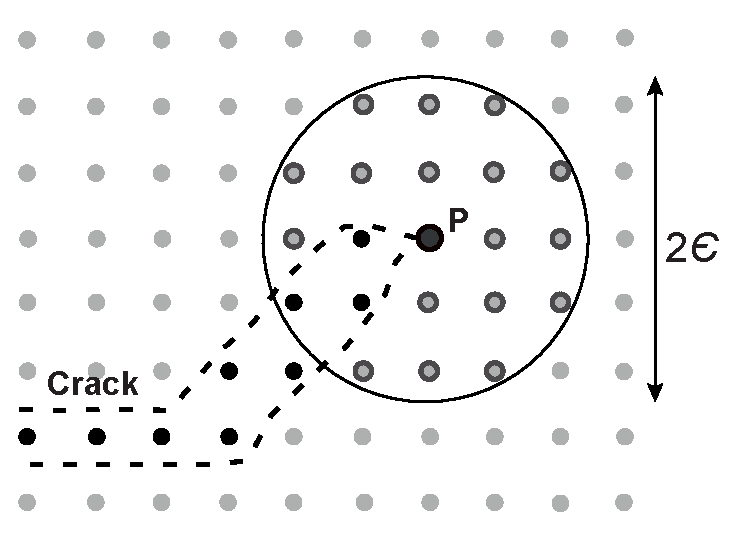
\includegraphics[width=0.44\textwidth]{Figs/eroded_neighbors_2.pdf}
\caption{Scheme of a fractured layer (black dots) as set of failed material points, and of the $\epsilon$-neighborhood (inside the circle) of the material point located at the crack tip (gray dots).}
\label{fig3}
\end{figure}
%%%%%%

On the other hand, the implementation of the eigensoftening algorithm consists in adopting a strength criterion for crack initiation and a softening law which is proper to the material under study before the formation of a stress-free crack. This second process tends to accumulate less energy until the crack. When the maximum tensile strength, $f_t$, is reached, a cohesive crack is formed with zero opening displacement. Once the opening displacement, $w$, reaches a critical vale, $w_c$, a stress-free crack is attained. The energy below the softening curve represents the static fracture energy per unit of area, $G_F$, which is sketched in Fig.~\ref{fig_GF}.
%%%%%%
\begin{figure}
\centering
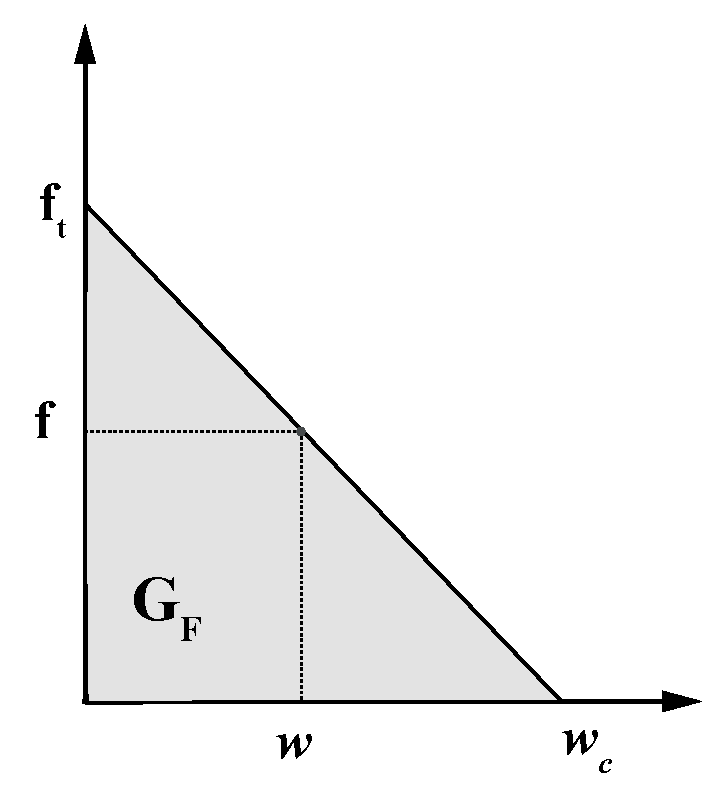
\includegraphics[width=0.44\textwidth]{Figs/GF.pdf}
\caption{Scheme of a linear cohesive law, where the shade area is $G_F$, $f_t$ is the tensile strength,  and $w_c$  is the critical opening displacement.}
\label{fig_GF}
\end{figure}
%%%%%%
For the Eigensoftening calculation, Eq.~(\ref{eq10}) can be rewritten in terms of the principal stresses at time $t_{k+1}$, since this model employs the first principal stress as a failure criterion. Therefore, the variation of the averaged strain energy density in the $\epsilon$-neighborhood of the material point $x_{p, k+1}$ can be expressed as,
%%%%
\begin{equation}\label{eq_Wp_1}
\delta W^\epsilon_{p} = \frac{\partial G_{p}}{C\epsilon} = \frac{1}{m_{p}}\sum_{x_{q}\in B_\epsilon (x_{p})} m_{q} \sigma_{q,1} \delta \varepsilon_q,
\end{equation}
%%%
where $\sigma_{q, 1}$ is the maximum principal stress at a neighboring material point $x_{q, k+1}$. Considering an effective strain $\varepsilon_q$ at the material point $x_{q, k+1}$, such that the variation of the local strain energy can be obtained as $\delta W_q = \sigma_{q, 1}\delta \varepsilon_q$, let assume the effective strain increment of each material point can be approximated by its counterpart in the neighborhood, being Eq.~(\ref{eq_Wp_1}) simplified as:
\begin{equation}\label{eq_Wp_3}
\delta W^\epsilon_{p}=\frac{\delta \varepsilon_p} {m_{p}} \sum_{x_{q,k+1}\in B_\epsilon (x_{p,k+1})} m_q \sigma_{q, 1}.
\end{equation}
Thus, the equivalent critical stress at the material point $x_{p, k+1}$ is defined as follows
%%%%
\begin{equation}\label{eq_sigmap}
\sigma^{\epsilon}_{p}=\frac{1}{m_{p}}\sum_{x_{q,k+1}\in B_\epsilon (x_{p,k+1})}m_q \sigma_{q, 1}
\end{equation}

When $\sigma^{\epsilon}_{p,k+1}$ surpasses the tensile strength, $f_t$,  the softening behavior is activated through the damage variable $\chi$, which ranges between zero (an intact material) and one (completely failed material points). Of course, $\chi$ depends on the current and critical opening measures, $w$ and $w_c$ respectively.  The latter is a material parameter, but the first one has to be measured in terms of the achieved strain and a length of affection called band width, $h_\epsilon$, equivalent to the crack band model of Ba\v{z}ant~\cite{Bazant83}. It bears emphasis that  a reference value for $h^{\epsilon}$ is between two and four times the maximum size of the aggregates for concrete according to Ba\v{z}ant~\cite{Bazant98}. Thus, this is a material parameter more than a numerical artifact. The relationship between strain and crack opening depends on the effective fracture strain, $\varepsilon^{\epsilon}_f$, defined as the difference between the strain at crack initiation, $\varepsilon_1(x_{p,0})$, and the current strain, $ \varepsilon_1(x_{p,k+1})$ for a material point $p$; and the band width as:

\begin{equation} \label{eq15}
 \varepsilon_f^{\epsilon} = \varepsilon_1(x_{p,k+1}) - \varepsilon_1(x_{p,0})  =  \frac{w}{h^{\epsilon}}
\end{equation}

\subsection{Eigendegradation model}
Following the work of Einav and Randolph~\cite{Zhang2015}, and the later implementations of Zhang~\textit{et al.}~\cite{Zhang2015} (similar also of some other implementations~\cite{Wang21,Singh21}), the behavior of sensitive clays can be modeled by strain softening curves in order to reduce the strength of the material by a degradation obtained by accumulation of strain. Einav and Randolph assumed that the current shear strength depends on the accumulated absolute shear strain, $\xi$, which is taken as a state variable from which an isotropic strength reduction, $\delta(\xi)$, is calculated as

\begin{equation} \label{eq16}
\delta(\xi)=s_{u} / s_{u i}=\delta_{\mathrm{rem}}+\left(1-\delta_{\mathrm{rem}}\right) \mathrm{e}^{-3 \xi / \xi_{95}}
\end{equation}
where
\begin{equation}\label{eq17}
\xi=\int_{t}\left|\dot{\gamma}_{\max }\right| \mathrm{d} t
\end{equation}

and $\left|\dot{\gamma}_{\max }\right|$ is the cumulative absolute shear strain, $s_{u}$ and $s_{u i}$ are the softened strength and initial strength, respectively, $\delta_{\text {rem }}$ is the fully remolded strength ratio, and $\xi_{95}$ is the cumulative shear strain required to cause $95 \%$ reduction (from peak to remolded). The assumption is that $\delta_{\text {rem }}$ may be taken as the inverse of the sensitivity of the soil, while an appropriate value for $\xi_{95}$ must be deduced from laboratory test data, or by conducting cyclic penetration and extraction tests with T-bar or ball.

The calculation of the cumulative shear strain can be achieved by the eigendeformation technique, departing from Eq.~\eqref{eq_Wp_1}, and considering, for the Eigendegradation calculation, that the stress remains constant in a neighborhood $\epsilon$. Thus, Eq.~\eqref{eq_Wp_1} can be simplified as

\begin{equation}\label{eq_Wp_4}
\delta W^\epsilon_{p}=\frac{\delta \tau_p} {m_{p}} \sum_{x_{q,k+1}\in B_\epsilon (x_{p,k+1})} m_q \gamma_{q},
\end{equation}

being $\delta \tau_p$ the increment of tangential stress of the neighborhood and $\gamma^{\epsilon}_{p}$ the current local shear strain, calculated as:

\begin{equation}\label{eq_Wp_5}
\gamma^{\epsilon}_{p}=\frac{1}{m_{p}}\sum_{x_{q,k+1}\in B_\epsilon (x_{p,k+1})}m_q \gamma_{q}
\end{equation}

Similarly, in the neighborhood $\epsilon$, the non-local cumulative strain of a material point $p$ is calculated, only when plasticity is activated, as follows:
\begin{equation}\label{eq18}
\xi^{\epsilon}_{p}=\int^{t_{k+1}}_{t_{p0}}\left|\dot{\gamma^{\epsilon}_{p}}\right| \mathrm{d} t
\end{equation}
being $t_{k+1}$ referred to the current step and $t_{p0}$ to the step when plasticity begins. 

Considering only shear failure, yield shear stress $\tau$ is equivalent to the softened strength, $s_u$, and the residual yield shear stress, $\tau_{95}$, can be reached by $\tau_{95}=\tau{rem}=s_{ui} \, \delta_{rem}$. Thus, in every state of degradation, the current yield shear stress, referred to the epsilon neighborhood, $\tau^{\epsilon}$, reads:

\begin{equation} \label{eq19}
\tau^{\epsilon}=\tau_{95}+\left(\tau_{i}-\tau_{95}\right) \mathrm{e}^{-3 \xi^{\epsilon}_{p} / \xi_{95}}
\end{equation}

It is remarkable that, in laboratory, parameter $\xi_{95}$ is not obtained. Instead, the displacement $\delta_{95}$ is achieves. In Fig.~\ref{fig_deg}.A) the degradation of the strength in terms of the displacement is plotted.
%%%
\begin{figure}
\centering
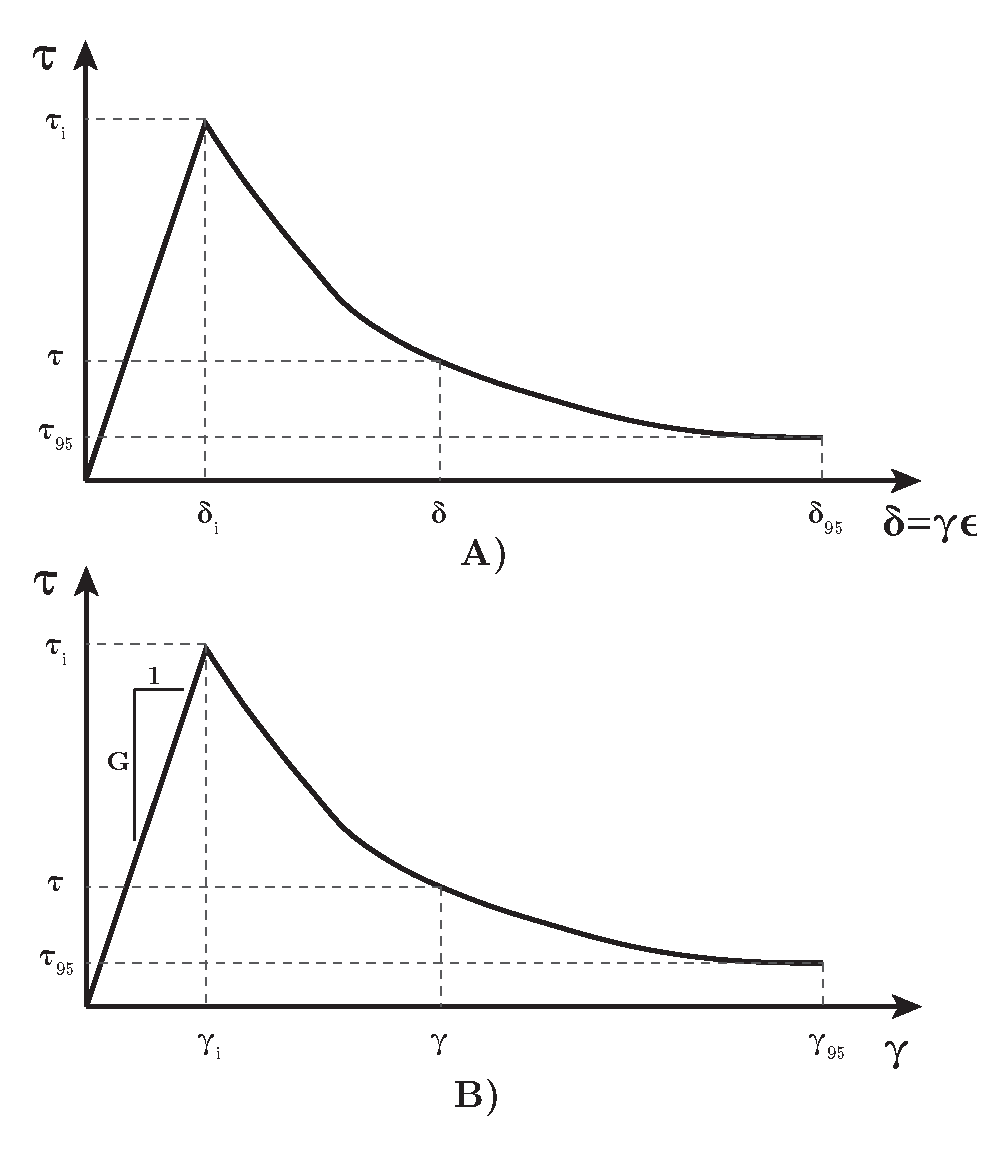
\includegraphics[width=0.44\textwidth]{Figs/degradation.pdf}
\caption{Degradation curve in terms of the displacement, A), and the shear strain, B).}
\label{fig_deg}
\end{figure}
%%%
 It can be seen how this law can be translated to the shear strain measurement (Fig.~\ref{fig_deg}.B) by multiplying by $\epsilon$, which, in this problem, is considered as the sliding length. Depending on the size of the soft layer, this parameter $\epsilon$ is obtained as the minimum length between the neighbor radius and the size of the soft layer (See Fig.~\ref{fig_layer}) as follows:
 \begin{equation} \label{eq20}
2\epsilon = \min(h_s,2C_\epsilon h)
\end{equation}
%%%
\begin{figure}
\centering
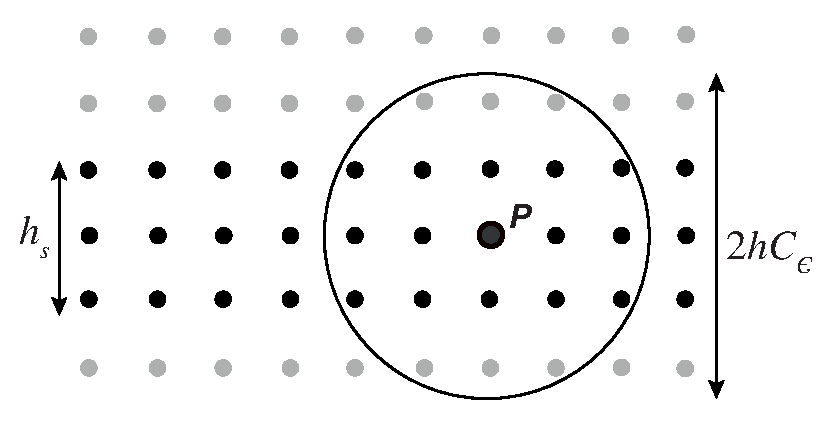
\includegraphics[width=0.44\textwidth]{Figs/soft_layer.pdf}
\caption{Scheme of the measurements of the soft layer (black dots) and the $\epsilon$-neighborhood around material point P.}
\label{fig_layer}
\end{figure}
\subsection{Visco-Plastic Eigendegradation algorithm}
Following, the pseudo-algorithm for the Eigendegradation model within a visco-plastic yield surface will be presented. It is worth mentioning that, prior to the algorithm steps, we need to calculate the equivalent shear total strain of every material point as the norm of the deviatoric total strain tensor. Since large strain is considered, the strain tensor is obtained through the logarithm of the left Cauchy-Green strain tensor, $\mathbf{b}$:

\begin{equation}\label{eq21}
\boldsymbol{\varepsilon}=\frac{1}{2}\log\boldsymbol{b}=\frac{1}{2}\log\boldsymbol{F F^T}.
\end{equation}

The aforementioned procedure can be followed in Algorithm~\ref{alg1}.

\begin{algorithm}
\caption{Visco-Plastic Eigendegradation algorithm}\label{alg1}
\begin{algorithmic}
\State \textbf{1. Calculation of the small strain tensor}
$$
\boldsymbol{\varepsilon}^{e\; trial}_{k+1}=1/2\,\log\mathbf{b}^{e\; trial}_{k+1}
$$
\State
\textbf{2. Elastic Predictor: volumetric and deviatoric stress measurements}
\begin{center}
Volumetric:  $p^{trial}_{k+1}=K \left(\varepsilon^{e}_{vol}\right)^{trial}_{k+1}$\\
Deviatoric:  $
\mathbf{s}^{trial}_{k+1}=2G\,\left(\boldsymbol{\varepsilon}^{e}_{dev}\right)^{trial}_{k+1}
$\\
\vspace{0.3cm}
being: $
\boldsymbol{\sigma}^{trial}_{k+1}=J^{-1}\boldsymbol{\tau}^{trial}_{k+1}
$\\
\vspace{0.3cm}
and:
$q^{trial}_{k+1}=\sqrt{\frac{3}{2}} \Vert \boldsymbol{s}^{trial}_{k+1} \Vert$
\vspace{0.15cm}
\end{center}
\textbf{3. Eigendegradation calculation}:\\
\IF {$t < t_{p0}$} $\qquad \sigma_y=\tau_i$
\ELSE
\begin{itemize}
\item
$
m_{p}=\sum_{x_{q,k+1}\in B_\epsilon (x_{p,k+1})}m_q
$
\vspace{0.15cm}
\item
$
\gamma^{\epsilon}_{p}=\frac{1}{m_{p}}\sum_{x_{q,k+1}\in B_\epsilon (x_{p,k+1})}m_q \gamma_{q}
$
\vspace{0.15cm}
\item
$
\xi^{\epsilon}_{p}=\sum^{k+1}_{k(t_{p0})} \left|\Delta\gamma^{\epsilon}(x_{p,k})\right| 
$
\vspace{0.15cm}
\item
$
\sigma_y=\tau_{95}+\left(\tau_{i}-\tau_{95}\right) \mathrm{e}^{-3 \xi^{\epsilon}_{p} / \xi_{95}}
$
\vspace{0.15cm}
\item Hardening modulus:
$
\qquad H=\frac{\partial \sigma_y}{\partial\overline{\varepsilon}^p} \simeq \frac{\partial \sigma_y}{\partial \xi^{\epsilon}_{p}} = -\frac{3\left(\tau_{i}-\tau_{95}\right)}{\xi_{95}} \mathrm{e}^{-3 \xi^{\epsilon}_{p} / \xi_{95}}
$
\end{itemize}
\ENDIF
\\
\vspace{0.3cm}
\textbf{4. Yield condition}: $\Delta\lambda=0$\\
\IF {$\phi= q^{trial}_{k+1} -\sigma_y \leq 0$} Elastic region: $\quad \boldsymbol{\sigma}_{k+1}=\boldsymbol{\sigma}^{trial}_{k+1}$
\vspace{0.3cm}
\ELSE    $\quad$  Viscoplastic flow:
\begin{itemize}
\item\textbf{4.1} Derivative of the yield surface:
\begin{equation}
d=\frac{\partial\phi}{\partial\Delta\lambda} = - \left( 3G  + \alpha \frac{q^{trial}_{k+1}  - 3G\Delta\lambda}{\Delta \lambda + \gamma\Delta t}\right) \left[  \frac{\gamma \Delta t}{\Delta \lambda+\gamma \Delta  t} \right]^{\alpha}  - H \nonumber
\end{equation}
\item\textbf{4.2} Increment of plastic strain:
$
\Delta\lambda=\Delta\lambda-\frac{\phi}{d}
$\vspace{0.3cm}
\item\textbf{4.3} Yield function:
$
\quad \phi= \left(q^{trial}_{k+1}  - 3G\Delta\lambda\right) \left[  \frac{\gamma \Delta t}{\Delta \lambda+\gamma \Delta  t} \right]^{\alpha} 
$\vspace{0.3cm}
\item\textbf{4.4} If $\phi < tolerance$ go to \textbf{4.5}, else go to  \textbf{4.1}
\item\textbf{4.5} Update
$$
\overline{\varepsilon}^p_{k+1}=\overline{\varepsilon}^p_{k}+\Delta\gamma
$$
$$
\Delta\boldsymbol{\varepsilon}_{k+1}^{p}= \frac{\Delta\gamma}{\|\textbf{s}^{trial}_{k+1}\|}\mathbf{s}^{trial}_{k+1}
$$
$$
\boldsymbol{\sigma_{k+1}}=\left(p^{trial}_{k+1} \right)\mathbf{I}+\left(1-\frac{3G\Delta\gamma}{q^{trial}_{k+1} }\right)\textbf{s}^{trial}_{k+1}
$$
\end{itemize}
\ENDIF\vspace{0.3cm}
%\algstore{myalg}
%\end{algorithmic}
%\end{algorithm}
%
%\begin{algorithm}
%\begin{algorithmic}
%\algrestore{myalg}
\State \textbf{5. Update elastic left Cauchy-Green Tensor}
$$
\boldsymbol{\varepsilon}_{k+1}^{e}= \boldsymbol{\varepsilon}^{e\; trial}_{k+1}-\Delta\boldsymbol{\varepsilon}_{k+1}^{p}
$$
$$
\mathbf{b}_{k+1}^{e}=\exp (2 \boldsymbol{\varepsilon}_{k+1}^{e})
$$
\end{algorithmic}
\end{algorithm}

%%%%%%%%%%%%%%%%%%%%%%%%%%%%%%%%%%%%%%%%%%
\section{Time and spatial discretization}
Following, the rest of computational tools that were employed in the present research are highlighted. First, the spatial discretization is shown, while the time discretization is mentioned in the final subsection.

\subsection{Spatial discretization}
The dynamic problem of a dry soil (mono-phase material) is studied in this research, being the time an important issue of the following analyses. The governing equation of the dynamic problem can be defined by the linear momentum balance equation:
\begin{equation}\label{eq_gov1}
 \mbox{div } \boldsymbol{\sigma}-\rho\boldsymbol{a}+\rho\boldsymbol{g}=\boldsymbol{0}.
\end{equation}
The derivation of the weak form of the problem needs the multiplication by the test function $\delta \boldsymbol{u}$, the virtual displacement, and the integration over the domain. After the application of the Green's Theorem, Equation \eqref{eq_gov1} yields:
\begin{eqnarray} \label{eq_gov1_a}
-\int_\Omega \boldsymbol{ \sigma} \, : \, \mbox{grad} \delta\boldsymbol{u} \,\, \differential{\Omega} + \int_{\Gamma_{t}} \delta\boldsymbol{u} \cdot\boldsymbol{\overline{t}} \, \differential \gamma - \int_\Omega \delta\boldsymbol{u} \cdot  \rho\boldsymbol{a}  \,\, \differential{\Omega} + \int_\Omega \delta\boldsymbol{u} \cdot 
\rho\boldsymbol{g}  \,\, \differential{\Omega}= 0 
\end{eqnarray}
where $\Omega$ represents the volume of the body and $\Gamma$ the boundary where tractions are applied. The first term of the equation is defined as the internal forces, meanwhile the second and forth conform the external forces. The next step is the interpolation through the Optimal Transportation Meshfree~\cite{li2010,li2014,Huang2019}, a meshfree method that has been demonstrated to perform reasonably well in geotechnical problems~\cite{Navas2020,Navas2021}. It is based in the conjunction of material points and nodes. As mentioned before, the shape functions are based on the work of Arroyo and Ortiz~\cite{arroyo2006}, who defined the Local Max-Ent shape function (LME) of the material point $\boldsymbol(x)$ with respect to the neighborhood $\boldsymbol(x_a)$ as follows:
\begin{equation} \label{eq_N1}
N_a(\textbf{x})=\frac{\exp\left[ -\beta__{LME} \; |\bf x-x_a|^2 +  \boldsymbol{\lambda}^*  \cdot  (x-x_a)  \right] } {Z(\textbf{x},\boldsymbol{\lambda}^*(\textbf{x}))},
\end{equation}
where the computation is done along a neighborhood $N_b$ and 
\begin{equation}\label{eq_N2}
Z({\bf x}, {\boldsymbol{\lambda}}) = \sum_{a=1}^{Nb}{ \exp \left[ -\beta__{LME} \, |{\bf x-x_a}|^2 + \boldsymbol{\lambda}  \cdot  \bf {(x-x_a)}         \right]}.
\end{equation}
The first derivatives of the shape function can be obtained from the own shape function and its Hessian matrix \textbf{J} by employing the following expression:
\begin{eqnarray}
\nabla N^*_a &=& -N^*_a \,  (\textbf{J}^*)^{-1} \,  (\bf x-x_a) \label{eq_N3} ,
\end{eqnarray}
The parameter $\beta__{LME}$ defines the shape of the neighborhood, and it is related with the discretization size (or nodal spacing), $h$,  and the constant, $\gamma__{LME}$, which controls the locality of the shape functions, as follows,
\begin{equation}\label{eqLM3}
\beta=\frac{\gamma__{LME}}{h^2}.
\end{equation} 

It bears emphasis that $\boldsymbol{\lambda}^*(\bf x)$ comes from the minimization of the function $g(\boldsymbol{\lambda})=\log Z(\bf x, \boldsymbol{\lambda})$ to guarantee the maximum entropy.\\

By employing the outlined shape functions and applying Galerkin procedure to the weak form, $\boldsymbol{u}$ can be interpolated by employing:
\begin{equation} \label{eq_uwp1}
\boldsymbol{u} \approx  \boldsymbol{u}^h = \boldsymbol{N}_u \cdot \tilde{ \boldsymbol{u} }
\end{equation}
where $\square^h$ represents the OTM approximation of the field $\square$ and $\tilde{ \square } $ the nodal values.  $\boldsymbol{N}_u = [N_1 \boldsymbol{I}, N_2 \boldsymbol{I}, ..., N_m \boldsymbol{I}]$ represents the shape function and $m$ is the number of nodes. Since the shape functions are defined in the reference configuration and time independent, $\boldsymbol{N} = \boldsymbol{N}(\boldsymbol{X})$, the following property holds:  $\dot{\square}^h =\boldsymbol{N} \cdot \dot{\tilde{\square}}$.
  
  \subsection{Time discretization}
  In this work, an implicit scheme has been proposed, since several applications cover a wide range of loading rates; from slow scenarios to quick phenomena. For the first ones, an explicit scheme would provide long computation time. Thus, the Newmark Implicit Scheme has been employed, with the parameters $\gamma=$0.6 and $\beta=$0.325 that are known to be suitable for dynamic problems~\cite{Kontoe2006}. To construct this scheme, Eq.~\eqref{eq_gov1_a} is reformulated as a system of equations, read as
\begin{equation}\label{eq_u1}
 \boldsymbol{ R}_{k+1}  +   \boldsymbol{M}   \, \boldsymbol {\ddot{u}}_{k+1}= \boldsymbol{P }_{k+1},
\end{equation}
where   $\boldsymbol{R}$ and $  \boldsymbol{ M}$ respectively denote the internal forces vector and mass matrix, whereas $ \boldsymbol{P}$ is the external forces vector, which contains both gravity acceleration and external nodal forces. ${k+1}$ represents the current step. Eq.~(\ref{eq_u1}) can be re-written with the Newmark scheme as:
\begin{eqnarray}\label{eq_u2}
\boldsymbol {G}_{k+1} &=& \boldsymbol {M}\left[\alpha_1\Delta\boldsymbol {u}_{k+1}-\alpha_2\boldsymbol {\dot{u}}_{k}-\alpha_3\boldsymbol {\ddot{u}}_{k}\right] +
+ \boldsymbol {R}_{k+1}-\boldsymbol {P}_{k+1}=\boldsymbol {0},
\end{eqnarray}

where the $\alpha$-parameters are listed in Table~\ref{tab1} according to Wriggers~\cite{wriggers:08}. These coefficients can be easily extended to any other time integration schemes. 
%%%
\begin{table}
\caption{\label{tab1} The $\alpha$-parameters of the Newmark scheme.} 
\centering
	%\vspace*{0.6cm}
	\begin{tabular}{lll}
	 $\alpha_1=\frac{1}{\beta\Delta t^2}$ & 	 $\alpha_2=\frac{1}{\beta\Delta t}$ & 
	 $\alpha_3=\frac{1}{2\beta}-1$
	\end{tabular}
\end{table}

Solving the above non-linear equations with a Newton-Raphson method, the resulting iterative scheme, taking into account the matrices that are involved in our problem, can be written as:
\begin{eqnarray}\label{eq_uw32}
\left[\alpha_1\boldsymbol {M}+\boldsymbol {K}^{i}_{k+1}\right]\Delta\boldsymbol{u}^{i+1}_{k+1} = \left[\boldsymbol {K_{*}}\right]^{i}_{k+1} \Delta\boldsymbol{u}^{i+1}_{k+1} &=& -\boldsymbol {G}(\boldsymbol {u}^{i}_{k+1}), \\
\mbox{where}\;\; \boldsymbol {u}^{i+1}_{k+1} &=& \boldsymbol {u}^{i}_{k+1} + \Delta \boldsymbol {u}^{i+1}_{k+1}.  \nonumber 
\end{eqnarray}
where $\boldsymbol {K}$ is the tangential stiffness matrix:
\begin{equation}\label{eq_uw31}
\boldsymbol {K}(\boldsymbol {u}^{i}_{k+1})=\boldsymbol {K}^{i}_{k+1}=\left.\frac{\partial\boldsymbol {R}}{\partial \boldsymbol {u}}\right|_{\boldsymbol{u}^{i}_{k+1}}.
\end{equation}
and $i$ depicts the iteration index. The iteration finishes when  $\boldsymbol {G}^{i}_{k+1}$ is smaller than a given tolerance.

%%%%%%%%%%%%%%%%%%%%%%%%%%%%%%%%%%%%%%%%%%
\section{Applications}
\label{S4}
Three tests have been studied in this research. The two first applications are devoted to show the performance of the two main principal properties of the proposed constitutive model: the degradation (Shear test, Sec.~\ref{S41}) and the viscous behavior (Strip footing load, Sec.~\ref{S42}). The last example shows the suitability of the model when the triggering and propagation of a slope due to cyclic loading is sought.

\subsection{Shear test}
\label{S41}
In the first example, the behavior of a weak layer under a shear test is analyzed. In Fig.~\ref{fig_geoshear} an embankment of 10 meters of depth is presented. A weak layer in the bottom of the domain of 0.5 meters appears. The proposed shear test is similar to the one proposed by Zhang \texit{et al.}\cite{Zhang2015}. Although different constitutive laws are employed (local and non-local), since both are based on similar degradation processes, it is expected to obtain comparable results.

The original embankment's length is 700 m. Since the softened zone only extends 90 m. and considering infinite conditions at both sides of this softened zone, only this 90 m. are modeled in order to save computational time. Unlike the original example, gravity conditions are neglected, considering the failure of the embankment at the final  of the residual strength. Thus, the parameters needed in this example are shown in Table~\ref{tab2}. It is important to point out that, in this research, the proposed non-local degradation model has been employed with a neighborhood parameter, $C_epsilon$, of 1.5. This is an important difference with the model proposed for the original example, which evaluates the degradation locally in an Arbitrary Eulerian-Lagrangian (ALE) configuration.

\begin{table}
\caption{\label{tab2} Parameters for the shear degradation analysis.} 
\centering
	%\vspace*{0.6cm}
	\begin{tabular}{ll}
	 Softened/modeled length $L=l_0$ & 	 90 m \\
	 Overall height, $H$ & 10 m \\
	 Height of sliding material, $h$ & 7.2 m \\
	 Shear band thickness, $s$ & 0.5 m \\
	 Submerged density of the soil, $\rho$ & 600 kg/m$^3$ \\
	 Poisson's ratio, $\nu$ & 0.495 \\
	 Young's modulus, $E$ & 1.98 MPa \\
	 Peak shear strength, $\tau_p=\tau_i$ & 10 kPa \\
	 Residual (95\%) shear strength, $\tau_{95}=\tau_r$ & 1.25 kPa \\
	 Plastic shear strain to 95\% reduction in strength, $\gamma_p$ & 0.6 \\
	 Neighborhood parameter, $C_\epsilon$ & 1.5
	\end{tabular}
\end{table}

\begin{figure}[!t]
\begin{center}
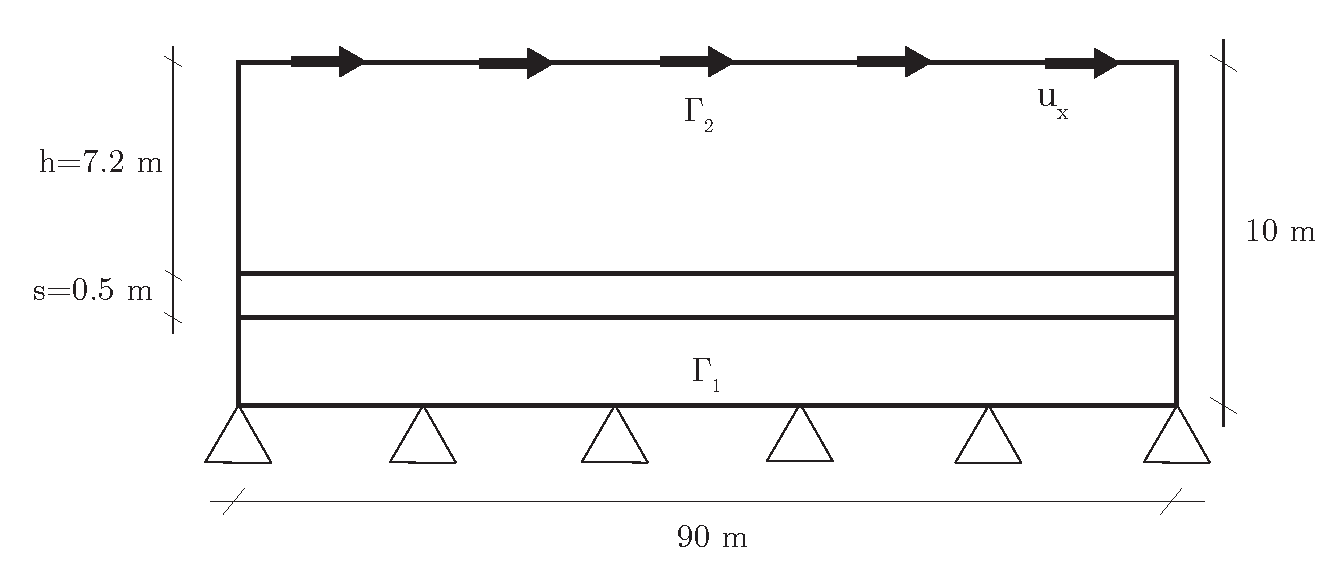
\includegraphics[width=12cm]{Figs/geo_shear.pdf}
\caption{Geometry and loading conditions of the shear degradation problem.}
\label{fig_geoshear}
\end{center}
\end{figure}

In addition, the geometry and boundary conditions can be seen in Fig.~\ref{fig_geoshear}. About the latest, two boundary conditions have been considered. In the first one, $\Gamma_1$ in Fig.~\ref{fig_geoshear}, both vertical and horizontal displacements are constrained. In $\Gamma_2$ a horizontal displacement of 10 meters is imposed gradually from 0 to 1000 s.

The stress behavior is analyzed in Fig.~\ref{fig_resshear}. In order to assess the performance of the proposed algorithm, similar to the figure proposed by Zhang \texit{et al.}\cite{Zhang2015}, in Fig.~\ref{fig_resshear} a dimensionless measurement of the shear stress is plotted. It is calculated as a relative increment from the residual shear strength $\tau_{95}$ and divided by the maximum increment, measured from the initial (or peak) strength to the residual one, $\tau_p-\tau_{95}$. On the other hand, in the abscissa, the dimensionless distance from the beginning of the degradation is plotted. Thus, the degradation starts from 0 until reaching the $\tau_{95}$ at distance 1. 

\begin{figure}[!t]
\begin{center}
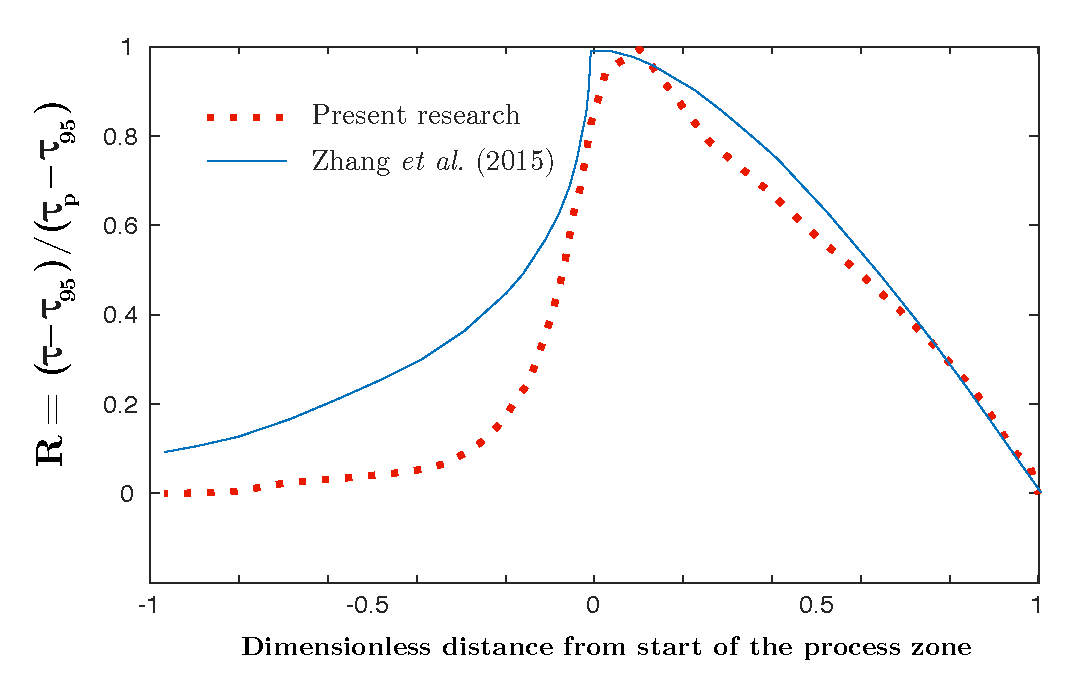
\includegraphics[width=12cm]{Figs/shear.pdf}
\caption{Geometry and loading conditions of the shear degradation problem.}
\label{fig_resshear}
\end{center}
\end{figure}

Results obtained in this research and the ones obtained by Zhang \texit{et al.}\cite{Zhang2015} are not coincident since they are different approaches; however, the overall trend, mainly after the beginning of the degradation, is similar to the reference research. This application allows us to assess the performance of a degraded layer of soft clay, which has been proved to perform similar to other validated studies.

\subsection{Strip footing load}
\label{S42}
Following, the behavior of the soil under different loading rates of a strip footing is analyzed. Similarly, the viscous properties of the soil are varied in order to extend the analysis to the behavior of the soil. This classic problem has been extensively used to verify the solutions provided by numerical models under viscoplastic conditions. The two main features to assess are the mechanism of failure and the behavior of the reaction forces at different viscoplastic scenarios. These results have been previously presented in the work of Pastor and coworkers \cite{BlancPastor2012,Navas2018}, where the loading is applied as an incremental velocity downwards at the base of the strip footing. In the present research, the loading is applied as a negative displacement according to the following expression: $$u_y=u_f\left(t/t_f\right)^2,$$ 
where $u_f=0.04$~m. and $t_f=4$~s. The geometry and soil parameters can be seen in Fig.\ref{fig_geozap}. Parameters of the Eigendegradation algorithm are also depicted. Opposite to the previous application, in this case there is no weak layer, acting the whole domain as a viscoplastic degradable soil.

%%%%%
\begin{figure}[!t]
\begin{center}
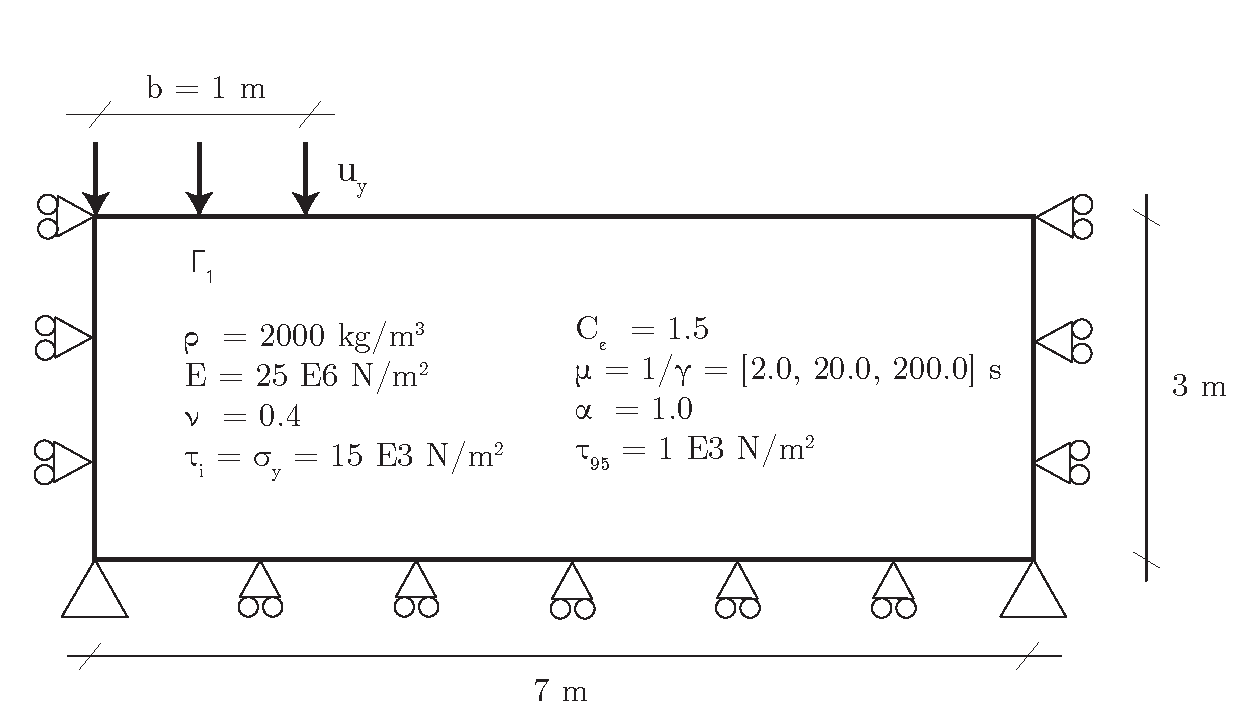
\includegraphics[width=12cm]{Figs/geo_zap.pdf}
\caption{Geometry, material parameters and loading conditions of the strip footing problem.}
\label{fig_geozap}
\end{center}
\end{figure}

The first calculation is made by activating the degradation part. This degradation acts as a softening of the material following the proposed exponential expression. It is known how the softening of the material boosts the formation of shear bands. In Fig.~\ref{fig_soft} the mechanism of failure is depicted. In~\cite{Navas2018}, there is a study of the influence of the discretization size and the parameters of the meshfree model. Optimal options achieved in the aforementioned study have been activated here.

\begin{figure}[!t]
\begin{center}
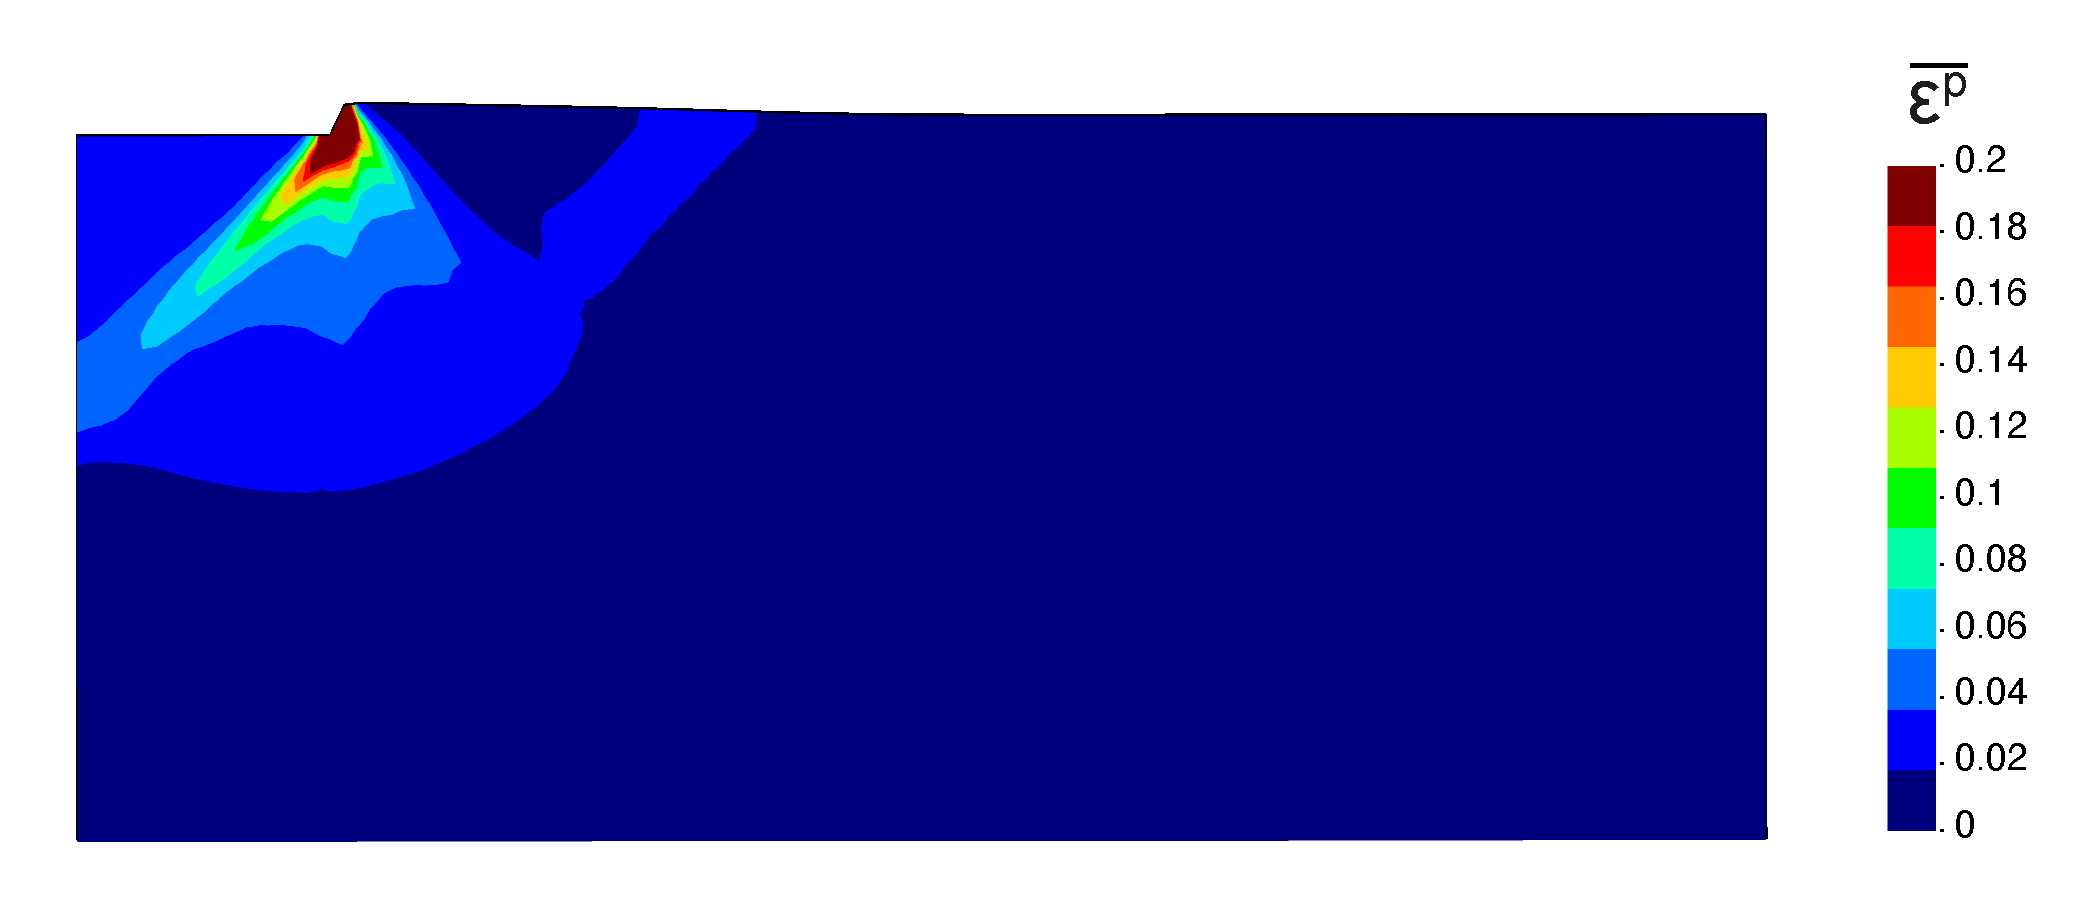
\includegraphics[width=12cm]{Figs/shear_band_foot.pdf}\\
\caption{Equivalent plastic deformation of the footing problem using von Mises law with softening through degradation at the final of the simulation.}
\label{fig_soft}
\end{center}
\end{figure}

In order to verify the performance of the full model, different viscous parameters have been employed in the calculation of the failure load of the strip footing. Establishing the sensitivity parameter $\alpha$ as 1.0, the viscous parameter has been varied with different values (see Fig.~\ref{fig_geozap}). The obtained results have been depicted in Fig.\ref{visco} for different values of $\mu$. The smaller the value of the $\mu$ parameter (\texit{i.e.} large values of $\gamma$), the higher the final loading is obtained from the footing loading, as expected from the viscous model. In addition, in dashed line, the reference value obtained by Navas \texit{et al.}~\cite{Navas2018} is depicted. This line can be considered as the value of a pseudo-static load is applied, without any rigidization due to the viscous behavior. This value is very close to the one obtained with $\mu=200$ s. 

\begin{figure}
\begin{center}
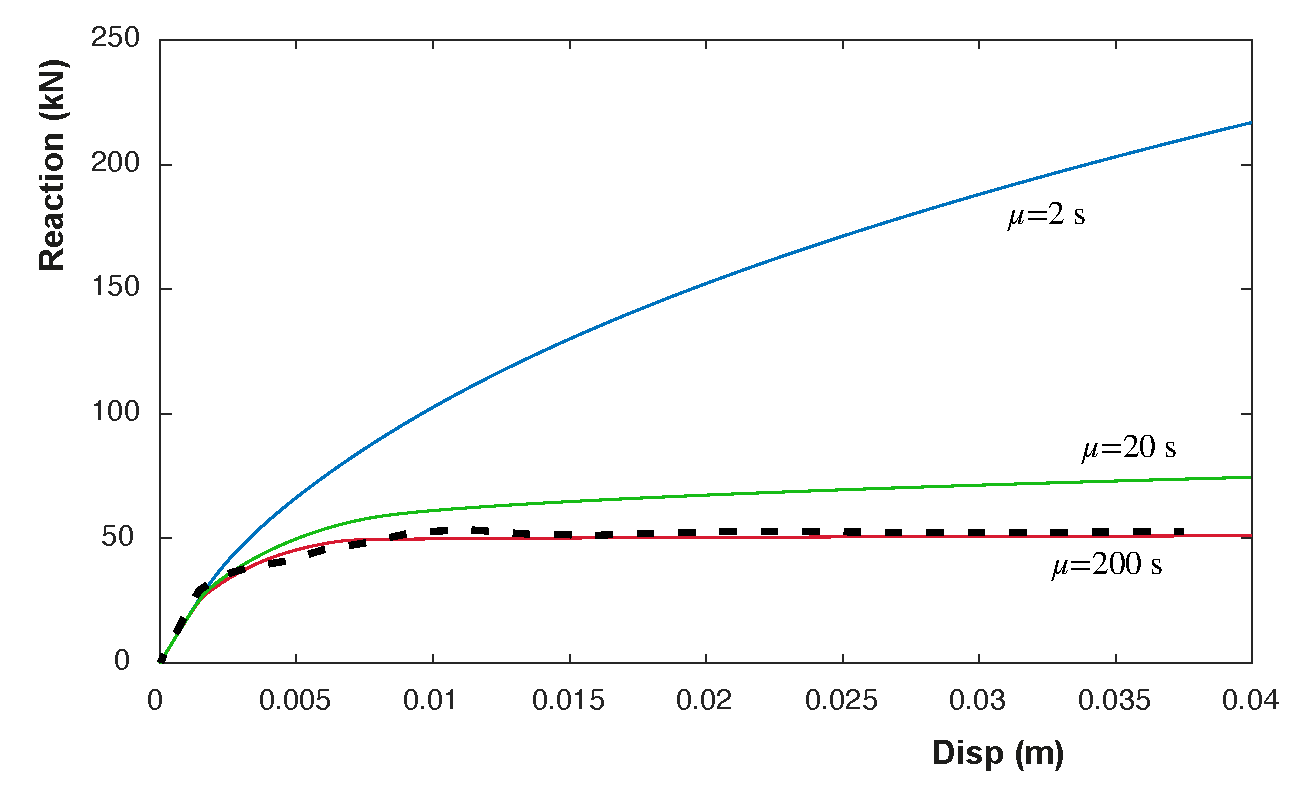
\includegraphics[width=11cm]{Figs/visco_d.pdf}\\
\caption{Obtained reaction with different $\mu$ values for the problem of the strip footing using viscoplastic von Mises law. The dashed line represents the pseudo-static behavior.}
\label{visco}
\end{center}
\end{figure}

Similarly, depending on the loading rate, the material can get stiffer and provide bigger response of the reaction forces. Thus, for $\mu=200$ s., 3 different loading rates have been tested. The obtained results have been depicted in Fig.\ref{visco2} for different values of $t_f$, being this parameter the final time of application of the imposed displacement ($u_y=u_f\left(t/t_f\right)^2$). The quicker is the application of the displacement, the higher the final loading is obtained from the footing loading, as expected from the viscous model. In addition, in dashed line, the reference pseudo-static value, obtained by Navas \texit{et al.}~\cite{Navas2018}, is depicted also in this figure, being close to the slowest case.

\begin{figure}
\begin{center}
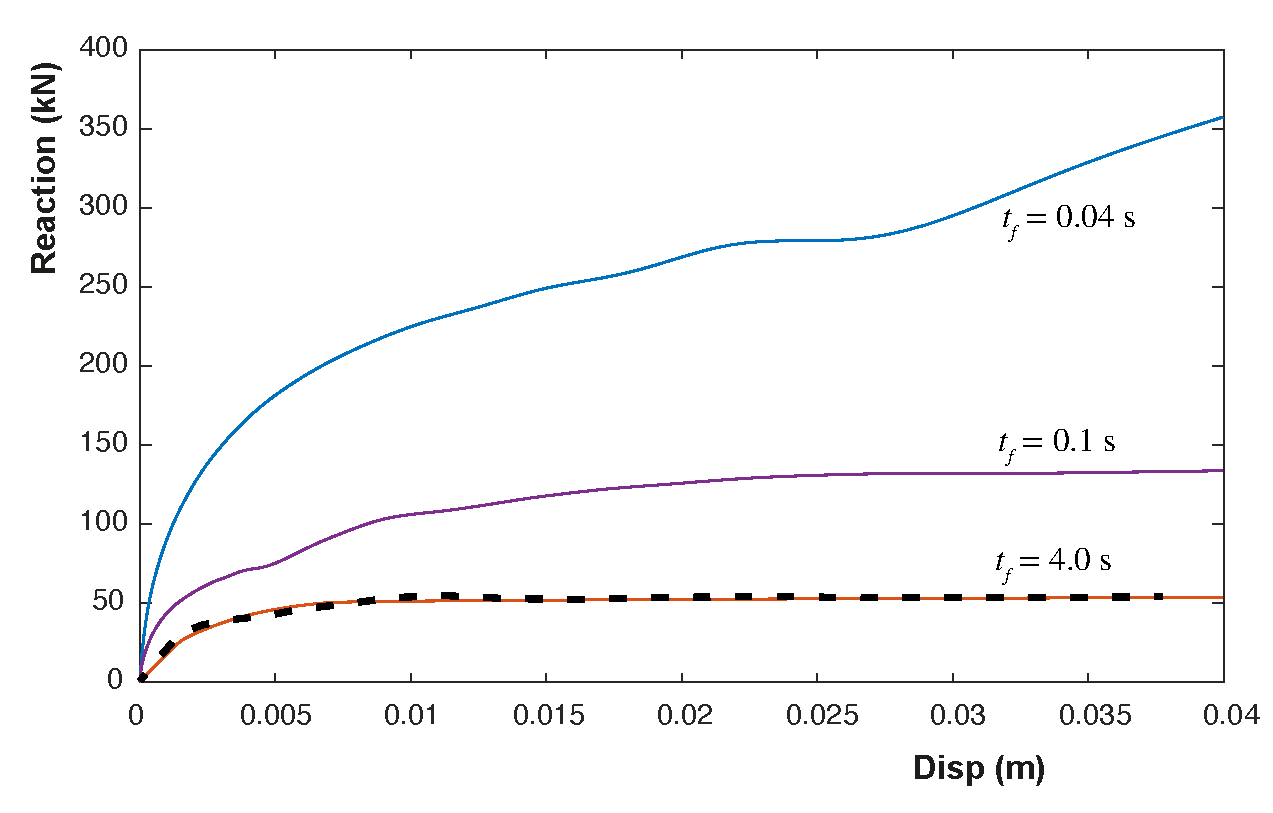
\includegraphics[width=11cm]{Figs/visco_t.pdf}\\
\caption{Obtained reaction with different loading rates for the problem of the strip footing using viscoplastic von Mises law, being $t_f$ the final time of the application of the load. The dashed line represents the pseudo-static behavior.}
\label{visco2}
\end{center}
\end{figure}

\subsection{Vertical cut}
This final application allows understanding the potentiality of the proposed methodology. A weak layer is supposed in a soil with a vertical cut on the left side. This weak layer is located forming a 45$^\circ$ angle, as it is sketched in Fig.~\ref{fig_VC1}. This layer, whose thick is 1 meter, will be considered plastic. Von Mises yield surface is employed, being its degradation modeled through both \emph{Eigendegradation} and traditional softening, in order to assess the performance of the first one against the latter. Out of the weak layer, the soil is considered elastic since its failure is far from the failure of the weak layer. Parameters of both models are presented in the right part of Fig.~\ref{fig_VC1}. In the traditional softening model, no Eigendegradation parameters are needed. Instead, a negative hardening of 200 kPa is employed. This parameter is not employed in the Eigendegradation simulation.

The soil can be considered infinite on the right and on the bottom of the model; thus, any movement in these directions is prevented. The 12 first meters are modeled for the sake of simplicity.

%%%
\begin{figure}
%\centering
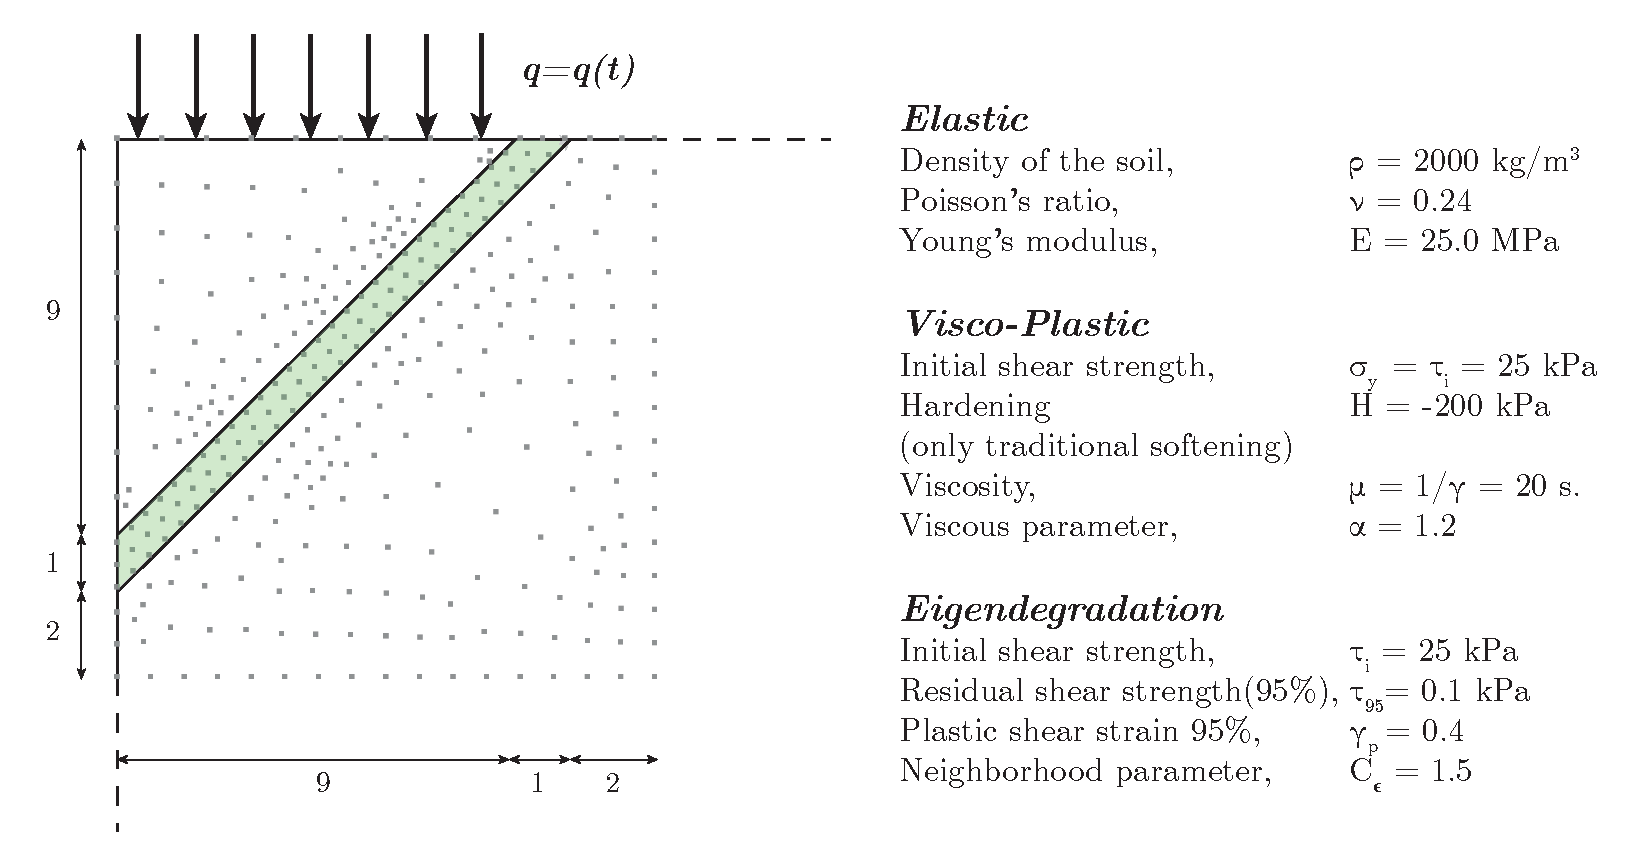
\includegraphics[width=0.75\textwidth]{Figs/geo_VC.pdf}
\caption{Left:Geometry of the vertical cut analyzed through \emph{Eigendegradation} and softening models and the location of the weak layer and the loaded zone. (Units in meters). Right: parameters of the employed models.} 
\label{fig_VC1}
\end{figure}
%%%

The top left part is loaded by a surface load, as it is shown in Fig.~\ref{fig_VC1}. This load is composed by two different waves, as it is sketched in Fig.~\ref{fig_VC2}.

%%%
\begin{figure}
%\centering
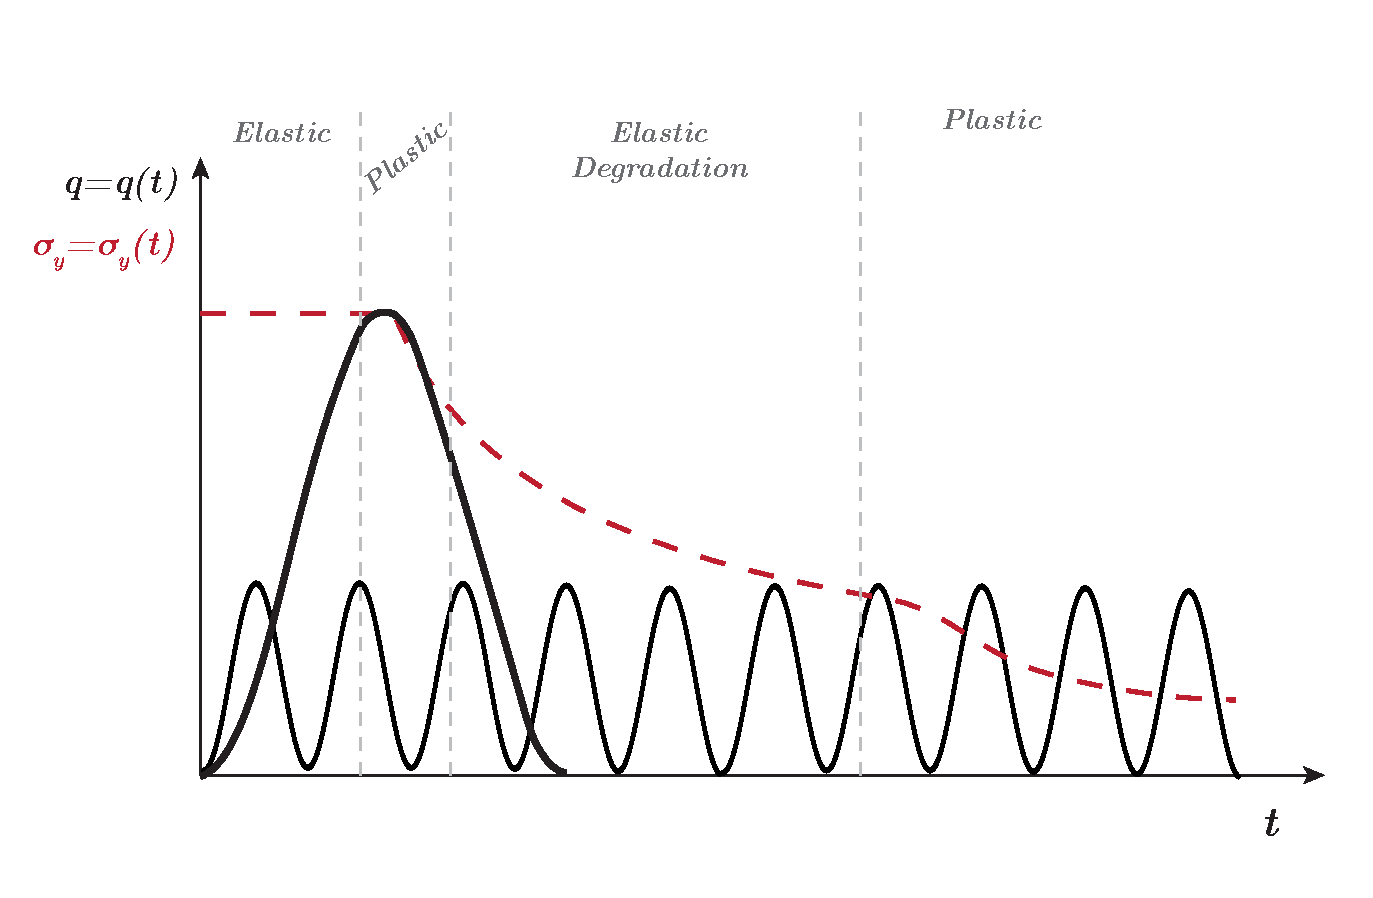
\includegraphics[width=0.7\textwidth]{Figs/carga_VC.pdf}
\caption{Scheme of the load and the yield strength along the time.}
\label{fig_VC2}
\end{figure}
%%%

Both waves follow the expression:
$$
q_\alpha(t)=A_{\alpha}\cdot\left[1-cos(\omega_{\alpha}t)\right]
$$

where $\alpha$ varies for each of both loads. The bigger load is the one that provokes the triggering of the plastic mechanism. It can be considered as an abnormal scenario that may lead to catastrophic consequences in the short or in the long time. Their parameters are $A_1=11$ kPa and $\omega_1=0.1\pi$ rad/s. This load is applied only in the first 20 seconds of simulation. The secondary load is of a lower magnitude. It could be considered as a usual load that the soil suffers permanently and is not capable to provoke the breakage of the slope by itself. The amplitude of this load is half of the first one, $A_2=5.5$ kPa and the frequency is much higher, $\omega_2=3\pi$ rad/s. This load is maintained through the 80 s. of the simulation.

Following, in Fig.~\ref{fig_VC3}, the evolution of both shear strength and the equivalent plastic strain are depicted along the time for both Eigendegradation and softening models. On the left, the shear strength is plotted. The first part of the figure is leaded by the first load: the material reach the yield stress close to 10 s. and start to decrease the strength till 15 s. Both materials, until this point, behave similarly. Observing the right figure, we can see how both models obtain plastic strain until 15 s. as well. Obviously, the amount of shear strain is different since one law is logarithmic (eigendegradation) and the other one is linear. After this point, the eigendegradation model accumulates shear strain (elastic in this case) that makes the shear strength to decrease. This elastic shear strain comes from the second law (the one with small amplitude). We know that is elastic strain since, in the right figure, no accumulated plastic strain is obtained from 15 s. to 50 s. From this point on, the equivalent plastic strain increases drastically. It is translated in an increment of the descent of the yield stress. However, since this accumulated strain provoked by the second load is elastic, no variation of the shear strength with the traditional softening model is observed. 

%%%
\begin{figure}
\centering
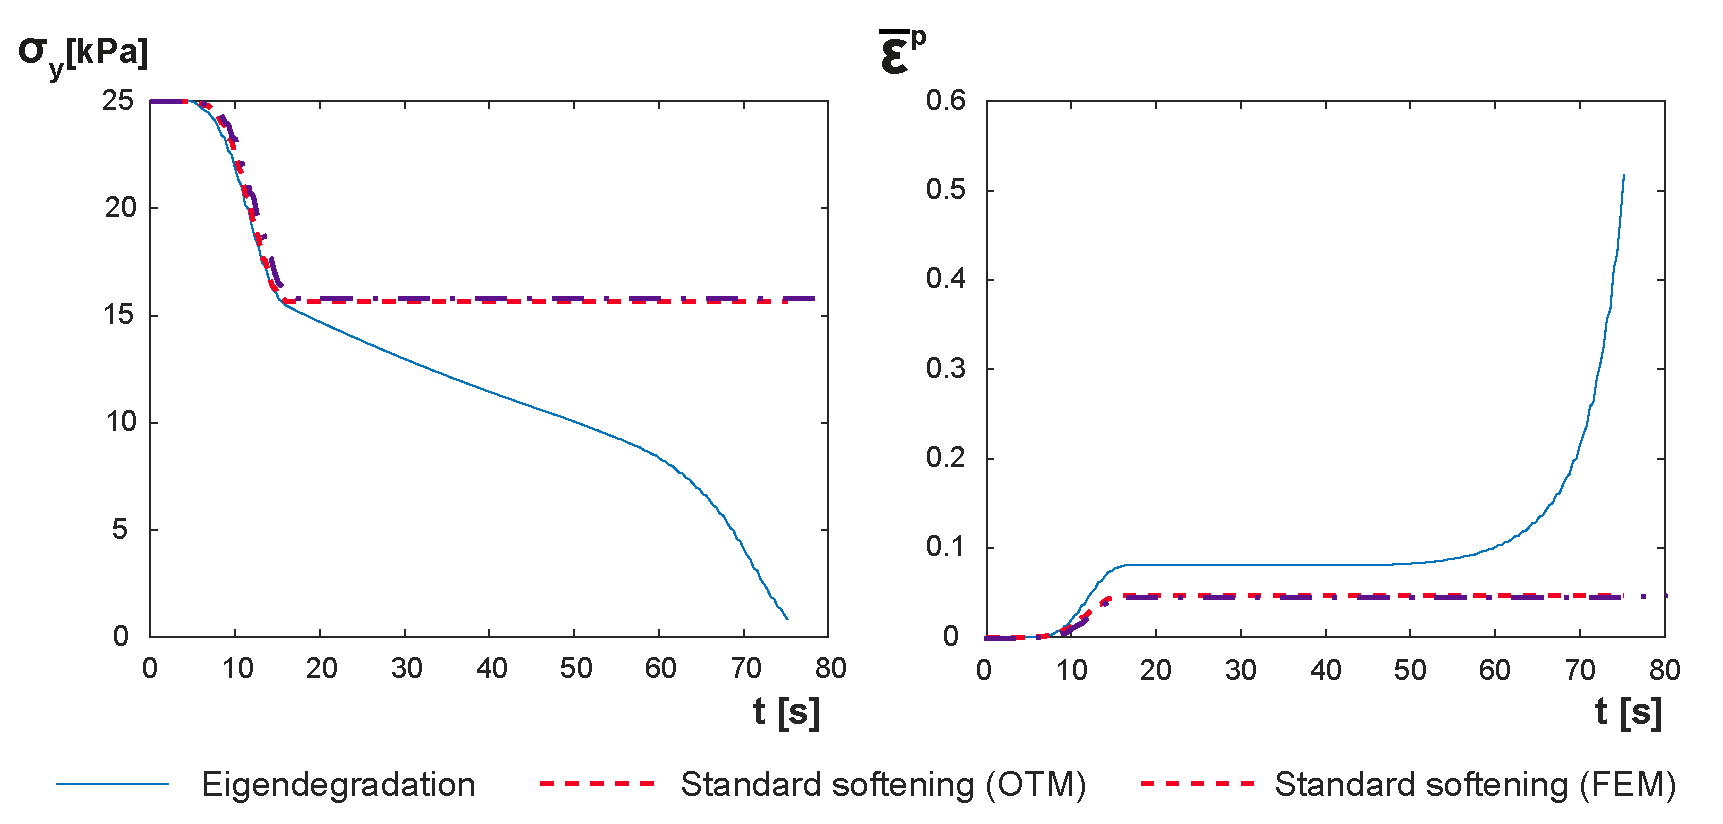
\includegraphics[width=0.75\textwidth]{Figs/evo_VC.pdf}
\caption{Evolution of the shear strength and the equivalent plastic strain along the time for both Eigendegradation and softening models.}
\label{fig_VC3}
\end{figure}
%%%

Another observation that arises from Fig.~\ref{fig_VC3} is the capability of the model of being sensitive to both loading and unloading conditions of the load, \textit{i.e.}, any variation of the strain, positive or negative, makes the material to degrade and lose shear strength. It is seen in the slope of the yield stress curve from 15 to 50 s., that remains constant along the whole loading cycle, equal in the loading or unloading branch.

Finally, in Fig.~\ref{fig_VC4}, the distribution of the equivalent plastic strain in the deformed model at 4 different times is depicted. The chosen moments were: i) the peak of the first load (around 15 s.), ii) the beginning of the secondary plastification of the material (50 s.), iii) moments before the failure of the slope (75 s.) and iv) moments after the triggering of the slope. 

%%%
\begin{figure}
%\centering
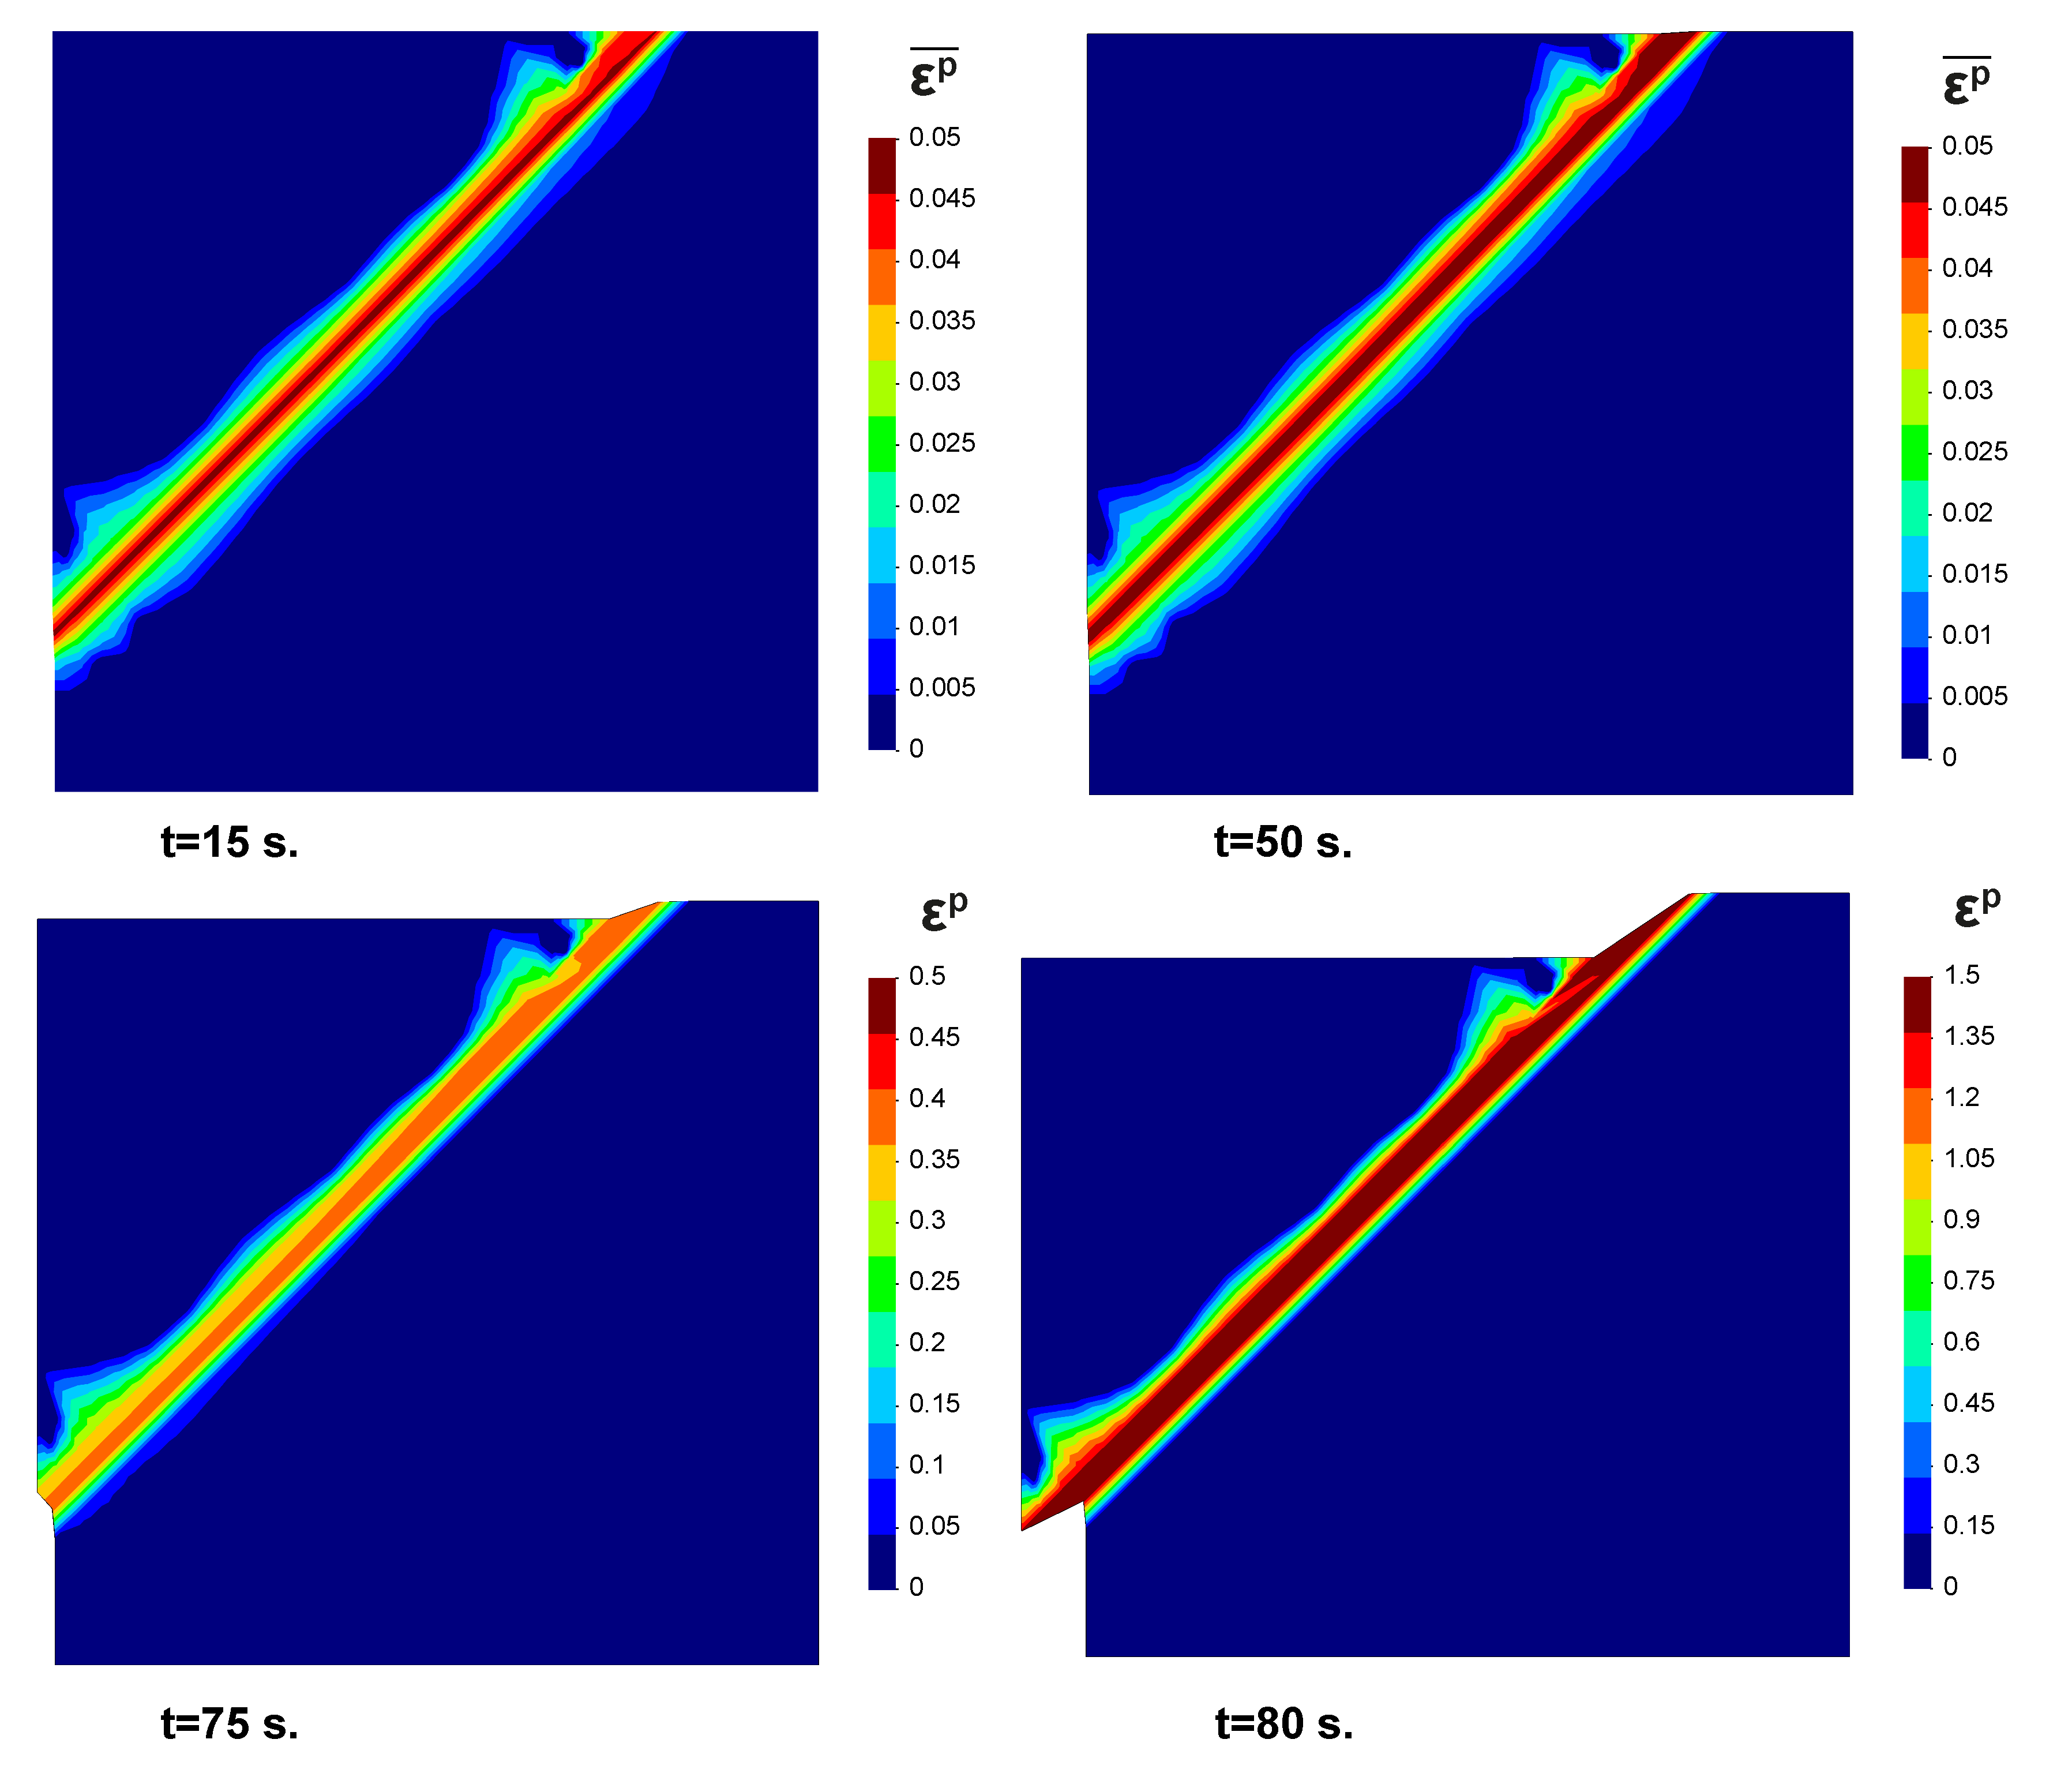
\includegraphics[width=0.7\textwidth]{Figs/EP_VC.pdf}
\caption{Distribution of the equivalent plastic strain in the deformed model at 4 different times.}
\label{fig_VC4}
\end{figure}
%%%

%%%%%%%%%%%%%%%%%%%%%%%%%%%%%%%%%%%%%%%%%%
\section{Conclusions}

A visco-plastic degradation model has been proposed in order to simulate the behavior of layers of soft clays. The non-local performance of the proposed algorithm has been carried out following concepts of non-local meshfree models capable to reproduce both brittle (Eigenerosion) and quasi-brittle (Eigensoftening) behaviors. Thus, the proposed algorithm takes the name of \textit{Eigendegradation}.

Two main properties defined the proposed constitutive model: softening due to degradation and visco-plastic behavior. Thus, two different examples are provided in order to validate both properties.

The first example reproduces a shear test of a soil with a thin soft layer. This test shows the performance of the degradation behavior from the beginning of the reduction of the shear strength to the final of this reduction, obtaining a residual strength. This result has been compared to other similar work of degradation of clays, obtaining very close curves,  what let us think the behavior of the proposed algorithm when modeling this material is correct.

The second example studies the behavior of a soil loaded by a strip footing. In this case, the viscoplastic concept is the one to be assessed. Since the von Mises yield surface is employed, the traditional Prandtl mechanism is obtained. Moreover, a hardening behavior is observed either when the viscosity becomes higher or when the load is applied quicker. This example allows us to validate the viscous behavior, as well as to verify that the degradation acts as a softening of the material that helps to define clearer the shear bands formed in the plastic mechanism.

Finally, a vertical cut of soil is modeled. This soil contains a 45$^\circ$ soft layer. A compound load is applied, being the first part what makes the beginning of the degradation of the material and the last part the one that makes the whole degradation of the shear strength and the final failure of the slope. In comparison with a traditional softening law, the proposed one is capable to produce degradation with elastic accumulated strain, being able the accumulation by both loading or unloading conditions. This behavior is seen in many failures of these kinds of soft layers, where a load much lower than the critical one but held in the time produces the fatigue of the material and the final failure of the soil structure. 

The present algorithm has performed successfully with the proposed applications. Further research can be made in order to be able to reproduce a wide range of problems. First of all, this model should be calibrated against experimental tests such as the shear test. Moreover, only the von Mises yield surface has been validated in this manuscript. Although it is able to reproduce the undrained conditions of the soil, more sophisticated yield surfaces, such as the Cam-Clay one, would improve the type of problems to be modeled. The soil should also be modeled as a biphase material, including the water in the formulation of the problem. Finally, some other spatial discretization, such as FEM or MPM, could be employed to assess the performance of this algorithm.

%%%%%%%%%%%%%%%%%%%%%%%%%%%%%%%%%%%%%%%%%%
\vspace{6pt} 


%%%%%%%%%%%%%%%%%%%%%%%%%%%%%%%%%%%%%%%%%%
\authorcontributions{Conceptualization, S. L\'opez-Querol. and D. Manzanal; software and validation, P.Navas; resources, A. Yag\"ue; supervision, M.Mart\'in-Stickle. All authors have read and agreed to the published version of the manuscript.}

\funding{This research was funded by the Ministerio de Ciencia e Innovaci\'on, under Grant Number, PID2019-105630GB-I00; and the European Research Council-H2020 MSCA-RISE, Grant Agreement No 101007851 (DISCO2-STORE), being both greatly appreciated.}

\acknowledgments{The administrative and technical support of both University College London and Universidad Polit\'ecnica de Madrid is greatly appreciated..}

\conflictsofinterest{The authors declare no conflict of interest.} 

%%%%%%%%%%%%%%%%%%%%%%%%%%%%%%%%%%%%%%%%%%
%% Optional
\abbreviations{The following abbreviations are used in this manuscript:\\

\noindent 
\begin{tabular}{@{}ll}
FEM & Finite Element Method\\
OTM & Optimal Transportation Meshfree\\
SPH & Smooth Particle Hydrodynamics\\
MPM & Material Point Method\\
ALE & Arbitrary Eulerian-Lagrangian
\end{tabular}}

%%%%%%%%%%%%%%%%%%%%%%%%%%%%%%%%%%%%%%%%%%
%% Optional
\vspace{6pt} 
\reftitle{References}

% Please provide either the correct journal abbreviation (e.g. according to the “List of Title Word Abbreviations” http://www.issn.org/services/online-services/access-to-the-ltwa/) or the full name of the journal.
% Citations and References in Supplementary files are permitted provided that they also appear in the reference list here. 

%=====================================
% References, variant A: external bibliography
%=====================================
\externalbibliography{yes}
\bibliography{lib2020}

%%%%%%%%%%%%%%%%%%%%%%%%%%%%%%%%%%%%%%%%%%
%% for journal Sci
%\reviewreports{\\
%Reviewer 1 comments and authors’ response\\
%Reviewer 2 comments and authors’ response\\
%Reviewer 3 comments and authors’ response
%}
%%%%%%%%%%%%%%%%%%%%%%%%%%%%%%%%%%%%%%%%%%
%\end{paracol}
\end{document}

